% This is LLNCS.DOC the documentation file of
% the LaTeX2e class from Springer-Verlag
% for Lecture Notes in Computer Science, version 2.4
\documentclass{llncs}
\usepackage{llncsdoc}

%
\usepackage{bm}
\usepackage{amsmath}

\begin{document}

\title{Anthropomorphic Finger Mechanism with a Nonelastic Bifurcate Tendon}
\author{Kazuya Yanagisawa, Shouhei Shirafuji, Shuhei Ikemoto, Koh Hosoda}
\institute{Information Science and Technology, Osaka University \email{yanagisawa.kazuya@ist.osaka-u.ac.jp}}
\maketitle

\begin{abstract}
 To realize both grasping stability and manipulation dexterity is a central
 problem in development of robot hands.
 % ロボットハンドにとってもっとも重要なのは,物体の安定把持と細かな操作を
 % 両立することである.
 In recent years, many underactuated robot hands have been developed to
 flexibly conform to an object's surface with a simple control system.
 % 近年,関節の数よりも少ないアクチュエータで駆動する劣駆動ハンドが多く開
 % 発され,一般的なロボットハンドに比べて簡単な制御で,物体表面に適応する
 % 柔らかな物体把持が実現されている.
 In contrast, it is difficult to realize dexterous manipulation which
 requires to control all degrees of freedom (DOFs).
 % しかし,劣駆動ハンドの場合には,アクチュエータの少なさから,細かな操作
 % を実現するのは難しい.
 In this research, we develop a robot gripper consists of two
 tendon-driven robot fingers with nonelastic bifurcate tendons to
 overcome the problem to realize dexterous manipulation by simple
 mechanism and control.
 % 本論文では,劣駆動のような簡易な制御で,細かい操作を実現するために,非
 % 伸縮な分岐腱をもつロボットフィンガで構成されたグリッパを開発することを
 % 目的とする.
 The bifurcate tendon indicates a tendon which branches and connect an
 actuator to different links.
 % 分岐腱とは,1つのアクチュエータにつながれた腱が,ある点で複数の腱に分岐
 % したものである.
 In particular, we focus on the nonelastic bifurcate tendon that
 connects an actuator to links of two DOFs robot finger.
 % ここでは,分岐腱構造としてもっとも単純な,2関節2腱のロボットフィンガを
 % 考える.
 In this robot finger, the displacement angles of the two joins are
 coupled by the nonelastic bifurcate tendon in the situation where no
 external force is exerted.
 % 分岐腱が非伸縮な場合,フィンガは,外力がない状態では,幾何学的な拘束に
 % より関節が連動して1自由度で動作する.
 If a certain amount of external force is applied on the fingertip, the
 bifurcate tendon can be slack and the coupling between two joints is
 broken.
 % 一方,フィンガの出す力や物体からの拘束といった条件によっては,分岐腱に
 % 緩みが生じ,関節の連動が生じなくなる.
 This means that the two DOFs robot finger is easily controlled as one
 DOF mechanism in reaching to an object, but it can still move by
 releasing the coupling provided by the bifurcate tendon while the
 fingertip is fixed on the object.
 % つまり,物体に接触するまでは,1自由度として簡易な制御で動作させることが
 % でき,指先が拘束されても,分岐腱を緩ませて関節の連動をなくすことでフィ
 % ンガの姿勢と指先位置を変化させ,把持後の物体操作を実現できる.
 Based on this idea, we develop and control the two DOFs robot finger
 that equipes two tendons including the nonelastic bifurcate tendon.
 % 以上をふまえ,2関節2腱のロボットフィンガを開発し,その制御を行った.
 In addition, we analyse the condition, where the bifurcate tendon gets
 slack, and confirmed in an experiment. 
 % さらに,分岐腱に緩みが生じるための力学的条件を考察し,実機で検証した.
 As the result, the availability of controlling the slack of bifurcated
 tendon was successfully confirmed.
 % その結果,意図的に分岐腱を緩ませる,もしくは緩ませないような制御ができ
 % ることを示した.
\end{abstract}

% \markboth{\LaTeXe{} Class for Lecture Notes in Computer
% Science}{\LaTeXe{} Class for Lecture Notes in Computer Science}
% \thispagestyle{empty}
% \begin{flushleft}
% \LARGE\bfseries Instructions for Authors\\
% Coding with \LaTeX\\[2cm]
% \end{flushleft}
% \rule{\textwidth}{1pt}
% \vspace{2pt}
% \begin{flushright}
% \Huge
% \begin{tabular}{@{}l}
% \LaTeXe{} Class\\
% for Lecture Notes\\
% in Computer Science\\[6pt]
% {\Large Version 2.4}
% \end{tabular}
% \end{flushright}
% \rule{\textwidth}{1pt}
% \vfill
% %\begin{flushleft}
% %\large\itshape
% %\begin{tabular}{@{}l}
% %{\Large\upshape\bfseries Springer}\\[8pt]
% %Berlin\enspace Heidelberg\enspace New\kern0.1em York\\[5pt]
% %Barcelona\enspace Budapest\enspace Hong\kern0.2em Kong\\[5pt]
% %London\enspace Milan\enspace Paris\enspace\\[5pt]
% %Santa\kern0.2em Clara\enspace Singapore\enspace Tokyo
% %\end{tabular}
% %\end{flushleft}
% \newpage
% %
% \section*{For further information please contact us:}
% %
% \begin{flushleft}
% \begin{tabular}{l@{\quad}l@{\hspace{3mm}}l@{\qquad}l}
% $\bullet$&\multicolumn{3}{@{}l}{\bfseries LNCS Editorial Office}\\[1mm]
% &\multicolumn{3}{@{}l}{Springer-Verlag}\\
% &\multicolumn{3}{@{}l}{Computer Science Editorial}\\
% &\multicolumn{3}{@{}l}{Tiergartenstra゚e 17}\\
% &\multicolumn{3}{@{}l}{69121 Heidelberg}\\
% &\multicolumn{3}{@{}l}{Germany}\\[0.5mm]
%  & Tel:       & +49-6221-487-8706\\
%  & Fax:       & +49-6221-487-8588\\
%  & e-mail:    & \tt lncs@springer.com    & for editorial questions\\
%  &            & \tt texhelp@springer.de & for \TeX{} problems\\[2mm]
% \noalign{\rule{\textwidth}{1pt}}
% \noalign{\vskip2mm}
% %
% %{\tt svserv@vax.ntp.springer.de}\hfil first try the \verb|help|
% %command.
% %
% $\bullet$&\multicolumn{3}{@{}l}{\bfseries We are also reachable through the world wide web:}\\[1mm]
%          &\multicolumn{2}{@{}l}{\texttt{http://www.springer.com}}&Springer Global Website\\
%          &\multicolumn{2}{@{}l}{\texttt{http://www.springer.com/lncs}}&LNCS home page\\
%          &\multicolumn{2}{@{}l}{\texttt{http://www.springerlink.com}}&data repository\\
%          &\multicolumn{2}{@{}l}{\texttt{ftp://ftp.springer.de}}&FTP server
% \end{tabular}
% \end{flushleft}


% %
% \newpage
% \tableofcontents
% \newpage
%

\section{Introduction} % (fold)
\label{sec:introduction}
Robot hands have been intensively studied to achieve humanlike stability
and dexterity in object manipulations.
% ロボットのエンドエフェクタ,特にロボットハンドの開発における目標の一つと
% して,ヒトの手のような物体の安定把持と細かな操作の両立があげられる.
During object manipulation, because a robot's body has to be controlled
at the same time as the control of the hand, to simplify the control to
reduce consumption of compuational resource is important.
% さらに,ロボットに実装する場合,ロボットの全身を同時に制御する必要からハ
% ンドに割ける計算能力には限界があるため,より簡便な制御でこれを実現するこ
% とも重要である.
There are two types of robot hands, which are to actuate joins by
motors implemented in the joints and to drive joints through tendons by
pulling them, in terms of hardware designs.
% ロボットハンドの駆動方式としては,関節を直接モータなどで駆動する方式と,
% 腱により駆動する方式がある.
In development of anthropomorphic robot hands, because to implement many
motors in each joints is space-consuming, the tendon-driven mechanism
has been often employed.
% 小型で,特にヒトを規範とするロボットハンドにおいては,関節にモータを組み
% 込むことの空間的な制約があること,また,ヒトの手を模倣するという観点から,
% 腱駆動を採用することがまず考えられる.
For instance, JPL/Stanford Hand\cite{Loucks1987}, Utah/MIT
Hand\cite{Jacobsen1986},and DLR-Hand\cite{Butterfass2001} are all
employing the tendon-driven mechanism.
% 腱駆動のロボットハンドとしては,JPL/Stanford Hand\cite{Loucks1987}や,
% Utah/MIT Hand\cite{Jacobsen1986},DLR-Hand\cite{Butterfass2001}などが有
% 名である.
In particular, ACT Hand\cite{Weghe2004} has the musculotendinous
structure which is very similar with that of humans.
% また,ヒトの手の構造を模倣したロボットハンドに,ACT Hand\cite{Weghe2004}
% がある.
Generally speaking, to realize dexterous object manipuation, robot hands
with many degrees of freedom (DOFs) is necessary.
% 一般に,物体の細かな操作を実現するためには,多くの自由度をもったロボット
% ハンドが必要になる.
In order for these tendon-driven hands to this end, however, many
tendons more than the number of joins (i.e. the number of DOFs) have to
be controlled.
% しかし,これらのロボットハンドのように腱駆動方式で制御するためには,関節
% の数,つまり自由度よりも多くの腱が必要になる.
Therefore, the number of actuators that the tendon-driven hands needs is
more than that of hands driven by motors implemented in each joints, and
the control becomes complex and difficult as the number of DOFs increases.
% そのため,自由度を保ったままハンドを駆動しようとすると,関節を直接駆動す
% る場合に比べてアクチュエータの数が増加してしまい,制御が複雑になるという
% 問題がある.

% To overcome this problem, in recent years, an approach to decrease
% complexity of control by designing a hardware which can bear a part of
% computaion in the control\cite{Pfeifer2010}.
% % この制御の複雑さという問題に対して,近年,制御の一部をロボットの機構や形
% % 態,もしくはシステムと環境との相互作用の中に取り込むことで制御の計算量を
% % 減らす方法が考えられている\cite{Pfeifer2010}.
% % 実環境で用いられるロボットは,常に環境からの影響を受けて動作している.
% % したがって,すべてを制御して目的の振る舞いをさせようとするのではなく,環
% % 境と相互作用することで目的の振る舞いをするような機構が注目されている.

To overcome this problem, the underactuated mechanism, which drives
joints by less number of actuators, has been researched\cite{Birglen2008}.
% このような形態への制御の取り込みとして,関節の数よりも少ないアクチュエー
% タでロボットを駆動する,劣駆動についての研究が進められている
% \cite{Birglen2008}.
For instance, Soft Gripper realized flexible encapsulation
grasping\cite{Hirose1978} and 100G Hand accomplished fast catching
task\cite{Kaneko2003}.
% 劣駆動のロボットハンドとしては,柔らかな包み込み把持を実現したSoft
% Gripper\cite{Hirose1978}を始めとし,高速なキャッチングが可能な100G
% Hand\cite{Kaneko2003}などがある.
In these hands, to employ passive mechanical elements such as springs
instead of actuators successfully simplify their structures and
controllers.
% これらのハンドでは,一部のアクチュエータの代わりにバネのような受動素子を
% 組み合わせることでアクチュエータの数を減らし,構造,制御を簡略化してい
% る.
Furthermore, passive mechanical elements are used to contribute flexible
grasping of an object by making the contact soft.
% さらに,受動素子を取り入れることで物体と接触したときには柔らかい把持を行
% えるように設計されている.
On the other hand, TUAT/Karlsruhe Hand, which has five underactuated
fingers consist of rigid linckages, realizes various types of
grasping\cite{Fukaya2013}.
% また,TUAT/Karlsruhe Hand\cite{Fukaya2013}では,ロッドの組み合わせにより
% 5指の劣駆動を行い,さまざまな姿勢の物体把持を実現している.
In contrast with these superior outcomes, however, underactuated hands
are often designed to be specialized for specific tasks, and the
mechanisms are difficult to achieve generality.
% しかし,劣駆動ハンドは,アクチュエータの少なさから,特定の機能を目的とし
% て設計することが多く,さまざまなタスクをこなせるハンドにはなりにくい.
For example, passive mechanical elements provide flexible object
grasping, but tasks such as in-hand manipulation, which require accurate
position control of fingertips, becomes difficult.
% また,受動素子のおかげで柔らかい物体把持を可能にする一方で,指先の細かな
% 位置制御などは難しくなり,物体をハンドの中で操作すると行った細かい動作を
% 実現している例は少ない.

Shirafuji et al. focused on the fact that the common digital extensor
tendon in a human hand branches before the PIP joint to propose a
mechanism for addressing the aforementioned problem, and developed the
3DOFs robot finger with the bifurcate tendon
structure\cite{Shirafuji2013}.
% このようにさまざまなハンドが開発されている中,Shirafuji et
% al.\cite{Shirafuji2013}は,ヒトの指の総指伸筋腱がPIP関節手前において分岐
% していることに着目し,そのモデルに基づきこの分岐腱構造を取り入れたロボッ
% トフィンガを開発した.
Since the bifurcate tendon is nonelastic, these branches connected to
different linckages are always tight, the geometric constraint provides
complete coupling of these two joints, and the 3DOFs structure can be
controlled as the 2DOFs mechanism.
% 分岐腱は伸縮せず,このフィンガは,指先に外力が働いていない状態では分岐し
% た腱がどちらも張っており,幾何学的な拘束から指先側の2関節が連動して動く.
% これにより,本来矢状面上で3自由度を持つ指を仮想的に2自由度で動かすことが
% できる.
In addition, in the condition where the fingertip touching to an object
receives a certain amount of external force, the coupling disappears by
making one of the branches slack.
% 対して,物体に接触し指先にある外力が働くと,フィンガの形態の変化により分
% 岐腱のどちらかに緩みが生じて関節が連動しなくなる.
Therefore, the finger controlled as the 2DOFs mechanism gets back in the
original 3DOFs structure thanks to the external force.
% そのため,2自由度で動いていた指は,物体の拘束を受けることで,元の自由度
% で動かすことができる.
As the result, they have shown that the structure with the nonelastic
bifurcate tendon can implicitly changes its DOF configuration.
% このように,分岐腱構造をもつフィンガは,明示的に制御することなくフィンガ
% の形態によって自由度を変化させることができる.

The idea of the nonelastic bifurcate tendon is thought of as applicable
for robot hands which are dexterous and easy to control.
% これらのことから,制御がしやすく物体操作に十分な自由度を持ったロボットハ
% ンドを開発するために,非伸縮な分岐腱をもつフィンガをロボットハンドに応用
% することが考えられる.
However, it is still not fully clarified how large external force and
tensions of tendons conduce the changes in the configuration, and how
the mechanism is applicable for object manipulation tasks.
% ただし,形態による自由度変化に必要な外力と腱張力の条件など,分岐腱をもつ
% ハンドについては研究されていないことも多く,構造の物体操作への寄与などの
% 有用性についても議論が進んでいない.
Therefore, it is necessary to investigate the advantages of the
mechanism by developing a simple robot hand exploiting the nonelastic
bifurcate tendon.
% そのため,分岐腱構造をもつロボットハンドとして簡単なシステムを実現し,そ
% の有用性を検証する必要があると考えられる.
So far, Sawada et al. has studied this kind of mechanism in terms of
position and stiffness of a robot arm
% また,分岐腱構造については,これ以前に,Sawada et al.\cite{Sawada2012}が,
% 分岐腱をもつアームにおける位置や関節剛性の制御について研究を行っている.
Their mechanism, however, employed elastic bifurcate tendon and did not
considered slack of the branch.
% しかし,Sawada et al.の扱っている分岐腱は弾性体であり,腱を緩ませること
% は想定されていない.
% したがって,自由度の変化は起こらないため,ここでは扱わない.

In this research, we develop a robot gripper consisting of 2DOFs fingers
with nonelastic bifurcate tendons to realize both stable grasping and
dexterous manipulation.
% 本論文では,分岐腱をもつロボットハンドにおいて物体の把持と操作を
% 実現することを目的とし,非伸縮な分岐腱を持つ2関節フィンガによる
% グリッパを開発する.
In this paper, at first, the developed 2DOFs finger and its position
control is presented.
% その前段階として,まず,分岐腱をもつ2関節2腱のフィンガを開発し,その位置
% 制御を行う.
In addition, we analytically investigate the condiion, where one of
branches of nonelastic bifurcate tendon looses, and confirm the
validity.
% また,分岐腱が緩むときの外力の条件について考察し,実機で検証を行うことで,
% 自由度変化の制御が可能であることを示す.
In the next, the robot gripper is developed by placing two developed
finger.
% その後,分岐腱により2関節が連動するフィンガを2本向かい合わせて固定し,グ
% リッパを製作する.
When these fingers are controlled by the same control signal, the
simplest robot gripper, which two fingertips similary move on sole
possible trajectory, is realized.
% 2本のフィンガを同時に同じ制御信号で駆動すると,ロボットハンドとしてもっ
% とも簡単な構造である,指先の軌道がある一定の曲線を描くグリッパを実現でき
% る.
In this design, the gripper simply opens/closes its fingers as 1DOFs
mechanism until stable grasping achieved, but the postures of fingers
can be changed for object manipulation by releasing fixed DOF.
% この構造により,物体を把持するまでは開閉のみの簡単な制御で把持を行い,把
% 持した後は2自由度として指の姿勢を変化させて物体を動かすことのできるグリッ
% パを実現できると考えられる.


\section{Robot finger with nonelastic bifurcate tendon} % (fold)
\label{sec:development}	
Fig.\ref{fig:coupled} shows the developed 2DOF robot finger driven by
two tendons.
% 本論文で,開発する2関節2腱のロボットフィンガのイメージを,図
% \ref{fig:coupled}に示す.
The finger has a nonelastic bifurcate tendon on the extensor aspect and
the antagonist tendon is located on the flexor aspect.
% フィンガは,伸展側に分岐腱をもち,屈曲側に拮抗に腱が存在する.
The two branches of the bifurcate tendon connected to two linckages over
two joints.
% 分岐腱は,分岐した後に2つの関節を通っており,分岐前には関節を通らない.
By reeling this tendon, these two joint are driven and they completely
engage while the branches are tight.
% これらの腱をアクチュエータで巻き取って駆動することで,腱が通っている関節
% にトルクが発生し,フィンガを動作させることができる.
% 特に,このように分岐腱が存在するフィンガにおいて,どの腱にも緩みが生じな
% いような状態で腱を駆動すると,分岐腱が関与する関節に連動が生じる.

% この分岐腱をもつ2関節2腱のロボットフィンガを開発し,制御することを考える.

%  % \begin{figure}[tb]
%  %  \centering
%  %  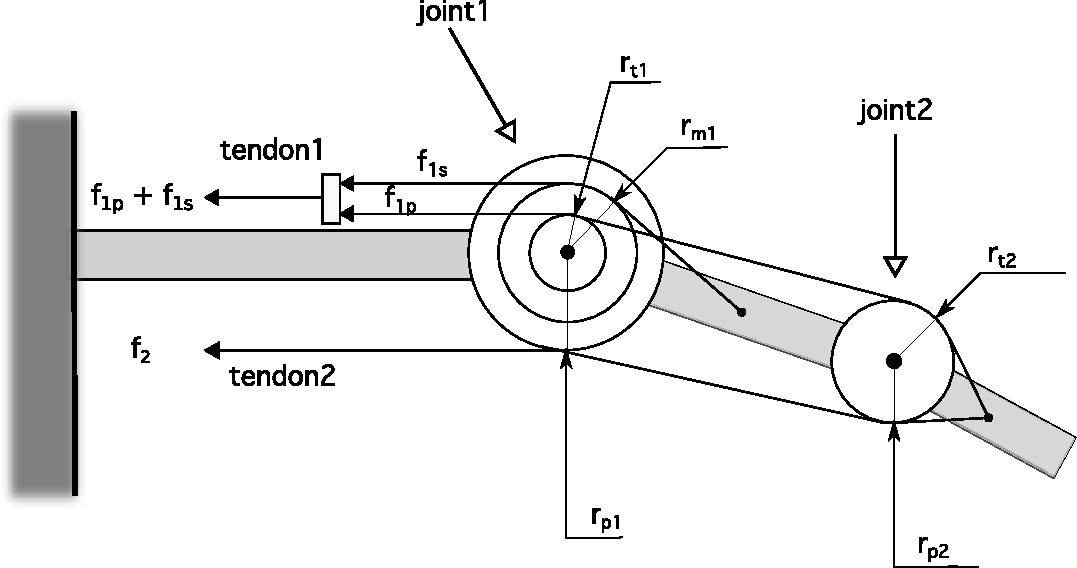
\includegraphics[width=.80\textwidth]{./figure/coupled.pdf}
%  %  \caption{分岐腱をもつ2関節2腱のロボットフィンガ}
%  %  \label{fig:coupled}
%  % \end{figure}

% 本章では,まず,一般的な腱駆動機構の運動学的表現と,分岐腱をもつ腱駆動機
% 構の運動学的表現について簡単に述べる.
% その後,実際に開発したロボットフィンガの詳細について述べる.


% \subsection{腱駆動機構における非伸縮分岐腱構造} 
%  \label{sub:branching_tendon}
% 関節を直接駆動するロボットの運動学は,関節角速度と手先の変位速度を関係づ
% けるヤコビアン行列を用いて表される.
% 腱駆動ロボットでは,これに加えて,腱の変位速度と関節角速度を関係づける腱
% ヤコビアン行列を用いて,運動が表現される.
% 分岐腱をもつロボットの場合,十分に緩みの生じない状態であるという仮定のも
% と,その幾何学的拘束により,この表現を簡略化することができる.
% 本節では,開発する2関節2腱のロボットフィンガを念頭に,腱駆動ロボットの運
% 動学的表現について述べた後,分岐腱をもつ場合にその表現がどのように変化す
% るか示す.

% \subsubsection{腱ヤコビアン} % (fold)
% \label{subsub:tendon_jacobian}
% 腱駆動ロボットフィンガの運動学的な表現を示す.
% Kobayashi et al.\cite{kobayashion1998}によると,腱駆動のロボットにおいて,
% 腱の移動速度$\bm{\dot{l}}$は,関節角速度$\bm{\dot{\theta}}$により,
		
% 		\begin{align}
% 		 \bm{\dot{l}} = \bm{J} \bm{\dot{\theta}},	\label{eq:l-theta}
% 		\end{align}
		
% 		と表される.
% 		ここで,$\bm{J}$は腱ヤコビアンであり,腱の各関節でのモーメントアームにより決定される行列である.

% 		さらにこの式と仮想仕事の原理により,各関節のトルク$\bm{\tau}$と腱の張力$\bm{f}$の間には,
		
% 		\begin{align}
% 		 \bm{\tau} = - \bm{J}^T \bm{f},	\label{eq:tau-f}
% 		\end{align}

% 		という関係が成立する.
% 		これより,腱ヤコビアン$\bm{J}$が正則であるとき,腱張力$\bm{f}$は,関節トルク$\bm{\tau}$用いて,

% 		\begin{align}
% 		 \bm{f} = - \bm{J}^{-T} \bm{\tau},	\label{eq:f-tau}
% 		\end{align}

% 		となる.
% 		しかし,実際のロボットフィンガでは,多くの場合において,腱ヤコビアンは正則ではない.
% 		このとき,$\bm{f}$は,次のように表される.

% 		\begin{align}
% 		 \bm{f} = - \bm{A}\bm{\tau} + \bm{f}_b.	\label{eq:f-tau-pinv}
% 		\end{align}

% 		ここで,$\bm{A}$は,$\bm{A} = \bm{J}(\bm{J}^T\bm{J})^{-1}$で表される$\bm{J}^T$の擬似逆行列である.
% 		$\bm{f}_b$は,$\bm{f}_b = (\bm{E} - \bm{A}\bm{J}^T)\bm{\xi}$で表されるバイアス腱張力である.
% 		$\bm{E}$は単位行列,$\bm{\xi}$は次元の一致する任意のベクトルである.
% 		式で表されるように,関節の数よりも多くの腱でフィンガを駆動する場合,$\bm{f}_b$で表されるような任意のバイアス張力を腱に加えることができる.
% 		このバイアス張力を変化させても,関節に発生するトルクは変わらない.
% 		また,腱駆動のロボットにおいては,腱で押すことはできないため,負の腱張力を発生させることはできない.
% 		そのため,腱を緩ませずにロボットを制御するためには,与えられた目標の関節トルクに対して,腱張力が正になるようなバイアス張力をかける必要がある.
% 		% (剛性について書くなら,アクチュエータと駆動軸間の非線形受動要素について言及が必要)
% 		% しかし,バイアス張力を多きくすればするほど,フィンガに外力を加えたときの動きに対する影響が小さくなる.
% 		% 逆に,バイアス張力が小さければ,外力の影響を非常に受けやすくなる.
% 		% したがって,こういったフィンガでは,関節の外力に対する動きにくさ,いわゆる剛性のようなものを自由に制御することができる.

% 		開発するフィンガにおけるヤコビアンを求める.
% 		分岐腱をそれぞれ独立の腱として考えると,2関節ロボットフィンガは図\ref{fig:finger}のようになる.
% 		ここで,関節角度,関節トルク,腱張力の各変数は,図中の矢印の向きを正とする.
% 		角度とトルクに関しては,フィンガが屈曲する向き,腱張力に関しては,腱が引っ張られる向きを正としている.
% 		また,図中には示していないが,腱の移動速度については,腱張力と同じく腱が引っ張られる向きを正とする.

% 		関節のトルクと腱張力の間の関係は,図より,各関節における腱のモーメントアームを用いて,

% 		\begin{figure}[tb]
% 		 \centering
% 		 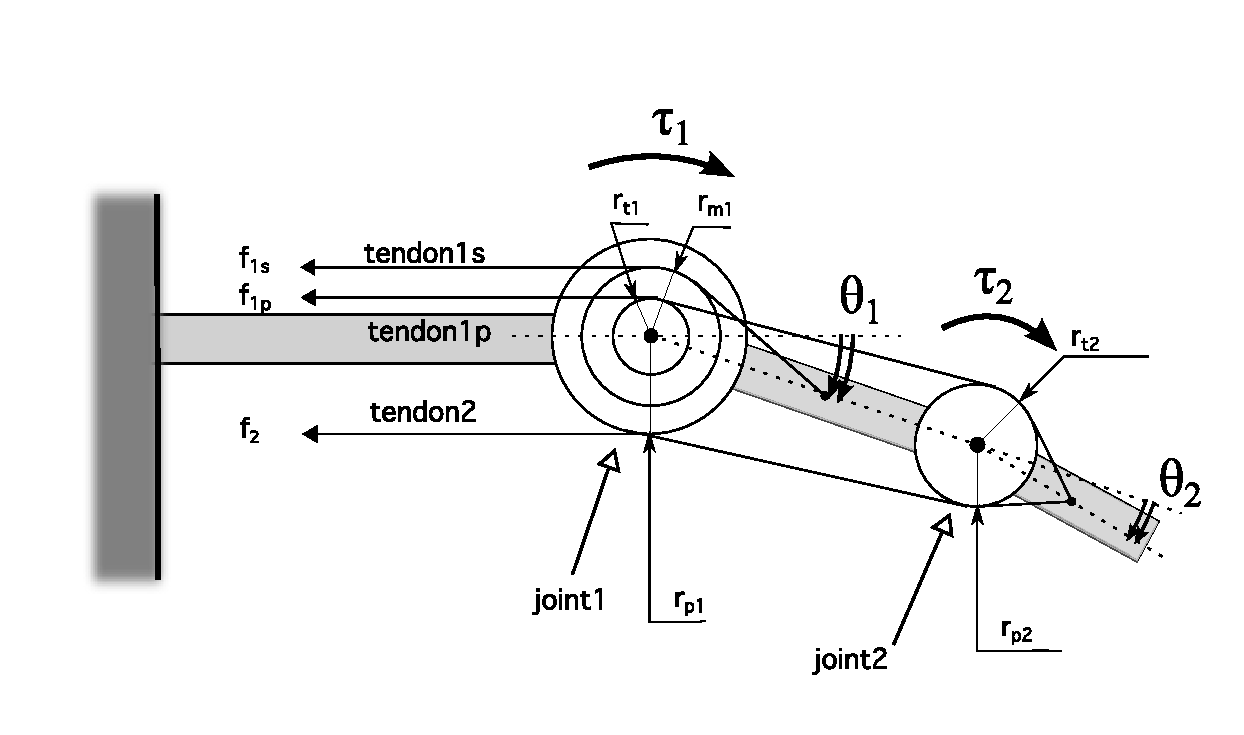
\includegraphics[width=.90\textwidth]{./figure/finger.pdf}
% 		 \caption{2関節2腱ロボットフィンガ}
% 		 \label{fig:finger}
% 		\end{figure}
		
% 		\begin{align}
% 		 \tau_1 & = r_{p1} f_2 - r_{t1} f_{1p} - r_{m1} f_{1s}, 	\label{eq:tau1-f-r}	\\
% 		 \tau_2 & = r_{p2} f_2 - r_{t2} f_{1p}, \label{eq:tau2-f-r}
% 		\end{align}
		
% 		という連立方程式として与えられる.
% 		$\tau_1,\tau_2$はそれぞれ,関節1,2におけるトルクであり,指が屈曲するときの方向を正とする.
% 				       これより,$\bm{\tau} = \begin{bmatrix}\tau_1 & \tau_2	\end{bmatrix}^T$,$\bm{f} = \begin{bmatrix}f_2 & f_{1p} & f_{1s}\end{bmatrix}^T$とおくと,式(\ref{eq:tau-f})から,$\bm{\tau}$と$\bm{f}$の関係を表す腱ヤコビアンが,次のように得られる.
				       
% 				       \begin{align}
% 					\begin{bmatrix}
% 					 \tau_1	\\
% 					 \tau_2
% 					\end{bmatrix} & = 
% 					\begin{bmatrix}
% 				 	 r_{p1} & - r_{t1} & - r_{m1} \\
% 				 	 r_{p2} & - r_{t2} & 0
% 					\end{bmatrix}\begin{bmatrix}
% 						      f_2	\\
% 						      f_{1p}	\\
% 						      f_{1s}
% 						     \end{bmatrix}.	\label{eq:Jt}	\\
% 					\bm{J} & = 
% 					\begin{bmatrix}
% 					 - r_{p1} & - r_{p2} \\
% 					 r_{t1} &  r_{t2} \\
% 					 r_{m1} & 0
% 					\end{bmatrix}.	\label{eq:J}
% 				       \end{align}
				       
% 				       この腱ヤコビアンを用いて,順運動学問題,逆運動学問題を考えることができる.
% 				       腱ヤコビアンから分かるように,腱駆動のロボットフィンガでは,各関節における腱のモーメントアームによって,腱張力と関節トルクの関係が変化する.
% 				       したがって,モーメントアームを変化させることにより,異なる動きのフィンガを設計することができる.

% 				       % subsection tendon_jacobian (end)

% 				       \subsection{分岐腱における仮想腱ヤコビアン} % (fold)
% 				       \label{sub:branching_tendon}
% 				       ロボットフィンガが,図\ref{fig:coupled}のような腱構造をもつ場合,式(\ref{eq:l-theta})を変形すると,

% 				       \begin{align}
% 					\begin{bmatrix}
% 					 \dot{l_{2}} \\
% 					 \dot{l_{1p}} \\
% 					 \dot{l_{1s}}
% 					\end{bmatrix} 
% 					& = 
% 					\begin{bmatrix}
% 					 \bm{J}_2 \\
% 					 \bm{J}_1
% 					\end{bmatrix} 
% 					\begin{bmatrix}
% 					 \dot{\theta_1} \\
% 					 \dot{\theta_2}
% 					\end{bmatrix}, \label{eq:l-theta_2joint}
% 				       \end{align}

% 				       が得られ,これを展開すると,

% 				       \begin{align}
% 					\begin{bmatrix}
% 					 \dot{l_{2}} \\
% 					 \begin{bmatrix}
% 					  \dot{l_{1p}} \\
% 					  \dot{l_{1s}}
% 					 \end{bmatrix}
% 					\end{bmatrix} 
% 					& = 
% 					\begin{bmatrix}
% 					 \bm{J}_2 
% 					 \begin{bmatrix}
% 					  \dot{\theta_1} \\
% 					  \dot{\theta_2}
% 					 \end{bmatrix} \\
% 					 \bm{J}_1
% 					 \begin{bmatrix}
% 					  \dot{\theta_1} \\
% 					  \dot{\theta_2}
% 					 \end{bmatrix}
% 					\end{bmatrix}, \label{eq:l-theta_branching}
% 				       \end{align}

% 				       という関係式が得られる.
% 				       $\dot{l_2},\dot{l_{1p}},\dot{l_{1s}}$はそれぞれ,腱2と,腱1が分岐したあとの,腱1p,腱1sの移動速度であり,$\dot{\theta_1},\dot{\theta_2}$は,関節1,2の角速度である.
% 				       ここで,$\bm{J}_2$は1×2行列,$\bm{J}_1$は2×2行列で,それぞれが腱2,1に対応する腱ヤコビアン$\bm{J}$の部分行列である.
% 				       \begin{align}
% 					\bm{J}_2 = 
% 					\begin{bmatrix}
% 					 - r_{p1} & - r_{p2}
% 					\end{bmatrix}, 
% 					\bm{J}_1 = 
% 					\begin{bmatrix}
% 					 r_{t1} &  r_{t2} \\
% 					 r_{m1} & 0
% 					\end{bmatrix}.	\label{eq:component_J}
% 				       \end{align}

% 				       ここで,腱の移動速度$\bm{\dot{l}} = \begin{bmatrix}
% 									    \dot{l_{2}} & \dot{l_{1p}} & \dot{l_{1s}}			
% 									   \end{bmatrix}^T $について,分岐した腱のどちらにも緩みがないときには,$\dot{l_{1p}} = \dot{l_{1s}}$が成り立つ.
% 									   これを用いて,式(\ref{eq:l-theta_branching})の腱1に関する部分を展開する.
% 									   まず,腱1に関する部分は,$\dot{l_{1p}} = \dot{l_{1s}}$のとき,

% 									   \begin{align}
% 									    \begin{bmatrix}
% 									     \dot{l_{1p}} \\
% 									     \dot{l_{1p}}
% 									    \end{bmatrix} 
% 									    & = 
% 									    \bm{J}_1
% 									    \begin{bmatrix}
% 									     \dot{\theta_1} \\
% 									     \dot{\theta_2}
% 									    \end{bmatrix},
% 									   \end{align}

% 									   と表される.
% 									   $\bm{J}_1$は,式(\ref{eq:component_J})より正則なので,逆行列が存在する.
% 									   よって,逆行列により,関節角速度$\dot{\bm{\theta}}$が計算でき,

% 									   \begin{align}
% 									    \begin{bmatrix}
% 									     \dot{\theta_1} \\
% 									     \dot{\theta_2}
% 									    \end{bmatrix} 
% 									    & = \dot{l_{1p}} \bm{J}_1^{-1} 
% 									    \begin{bmatrix}
% 									     1 \\
% 									     1
% 									    \end{bmatrix}, \label{eq:theta_coupled}
% 									   \end{align}

% 									   となる.
% 									   ここで,式(\ref{eq:component_J})より,$\bm{J}_1$をモーメントアームを用いて表すと,$\dot{\bm{\theta}}$は,

% 									   \begin{align}
% 									    \begin{bmatrix}
% 									     \dot{\theta_1} \\
% 									     \dot{\theta_2}
% 									    \end{bmatrix} 
% 									    & = - \frac{\dot{l_{1p}}}{r_{m1}r_{t2}}
% 									    \begin{bmatrix}
% 									     0 & -r_{t2} \\
% 									     -r_{m1} & r_{t1}
% 									    \end{bmatrix}
% 									    \begin{bmatrix}
% 									     1 \\
% 									     1
% 									    \end{bmatrix}, \\
% 									    \begin{bmatrix}
% 									     \dot{\theta_1} \\
% 									     \dot{\theta_2}
% 									    \end{bmatrix} 
% 									    & = \frac{\dot{l_{1p}}}{r_{m1}}
% 									    \begin{bmatrix}
% 									     1 \\
% 									     \frac{r_{m1}-r_{t1}}{r_{t2}} \label{eq:branching_theta}
% 									    \end{bmatrix},			
% 									   \end{align}

% 									   と計算できる.

% 									   以上より,2関節2腱のグリッパで分岐腱が連動しているとき,関節2と関節3の間の角速度の間に,
									   
% 									   \begin{align}
% 									    \dot{\theta_1} : \dot{\theta_2} = 1 : \frac{r_{m1}-r_{t1}}{r_{t2}}, \label{eq:rate_theta}
% 									   \end{align}
									   
% 									   という比例関係があることがわかる.
% 									   また,式(\ref{eq:branching_theta})の右辺に含まれる時間に依存する項は$\dot{l_{1p}}$のみであるので,関節の角度についても,初期姿勢の角度の値を上手く定義することで,同様の比例関係が成り立つ.

% 									   このように,分岐腱をもつロボットフィンガにおいては,分岐腱に緩みがなければ,分岐腱が関与する関節は,連動することが分かる.
% 									   したがって,関節を連動させた状態で制御したい場合には,分岐腱が緩まないように注意する必要がある.
% 									   この分岐腱が緩む条件については,後述する.
% 									   % 特に,腱に張力がかかっているフィンガが物体に接触しておらず,外力が働いていない場合,腱は緩まないため,関節の連動が必ず生じる.

% 									   この連動が生じているとき,$\dot{\bm{\theta}}$は,上述のように,式(\ref{eq:theta_coupled})で表される.
% 									   これを,式(\ref{eq:l-theta_2joint})の$\dot{\bm{\theta}}$に代入し式を変形すると,

% 									   \begin{align}
% 									    \begin{bmatrix}
% 									     \dot{l_{2}} \\
% 									     \dot{l_{1p}} \\
% 									     \dot{l_{1s}}
% 									    \end{bmatrix} 
% 									    & = 
% 									    \begin{bmatrix}
% 									     \bm{J}_2 \\
% 									     \bm{J}_1
% 									    \end{bmatrix} 
% 									    \dot{l_{1p}} \bm{J}_1^{-1} 
% 									    \begin{bmatrix}
% 									     1 \\
% 									     1
% 									    \end{bmatrix}, \label{eq:leading_Jc}	\\	
% 									    % \begin{bmatrix}
% 									    % 	\dot{l_{2}} \\
% 									    % 	\dot{l_{1p}} \\
% 									    % 	\dot{l_{1s}}
% 									      % \end{bmatrix} 
% 									    %  & = \dot{l_{1p}}
% 									    %  \begin{bmatrix}
% 									    %  	\bm{J}_2 \bm{J}_1^{-1} 
% 									    %  \begin{bmatrix}
% 									    % 	1 \\
% 									    % 	1
% 									       %  \end{bmatrix}	\\
% 									    %  	\bm{J}_1 \bm{J}_1^{-1} 
% 									    %  \begin{bmatrix}
% 									    % 	1 \\
% 									    % 	1
% 									       %  \end{bmatrix}
% 									       %  \end{bmatrix}, \\
% 									    \begin{bmatrix}
% 									     \dot{l_{2}} \\
% 									     \begin{bmatrix}
% 									      \dot{l_{1p}} \\
% 									      \dot{l_{1s}}
% 									     \end{bmatrix}
% 									    \end{bmatrix} 
% 									    & = \dot{l_{1p}}
% 									    \begin{bmatrix}
% 									     \bm{J}_2 \bm{J}_1^{-1} 
% 									     \begin{bmatrix}
% 									      1 \\
% 									      1
% 									     \end{bmatrix}	\\
% 									     \begin{bmatrix}
% 									      1 \\
% 									      1
% 									     \end{bmatrix}
% 									    \end{bmatrix},
% 									   \end{align}

% 									   となる.
% 									   右辺の行列において,腱1に相当する下側2行は線形従属となっている.
% 									   これをまとめた行列を$\bm{J}_c$とおくと,

% 									   \begin{align}
% 									    \bm{J}_c &= 
% 									    \begin{bmatrix}
% 									     \bm{J}_2 \bm{J}_1^{-1}
% 									     \begin{bmatrix}
% 									      1 \\
% 									      1
% 									     \end{bmatrix} \\
% 									     1
% 									    \end{bmatrix},
% 									   \end{align}

% 									   となる.
% 									   この行列$\bm{J}_c$を,仮想腱ヤコビアンと呼び,分岐腱をもつロボットフィンガにおいて,その運動を記述する際に用いることができる.

% 									   この仮想腱ヤコビアンを,式(\ref{eq:tau-f})においても利用することを考える.
% 																												 式(\ref{eq:tau-f})のヤコビアン$\bm{J}$を,$\bm{J}_c$に変換するためには,式(\ref{eq:leading_Jc})における操作と同様に,ヤコビアンに右から$(\bm{J}_1^{-1}\begin{bmatrix}1 & 1\end{bmatrix}^T)^T$をかければよい.
% 																																   したがって,$(\bm{J} \bm{J}_1^{-1}\begin{bmatrix}1 & 1\end{bmatrix}^T)^T = \begin{bmatrix}1 & 1\end{bmatrix} \bm{J}_1^{-T} \bm{J}^T$より,式(\ref{eq:tau-f})の両辺に左から$\begin{bmatrix}1 & 1\end{bmatrix} \bm{J}_1^{-T}$をかけると,

% 																																   \begin{align}
% 																																    \begin{bmatrix}
% 																																     1 & 1
% 																																    \end{bmatrix} \bm{J}_1^{-T} \bm{\tau} &= - \begin{bmatrix}
% 																																						1 & 1
% 																																					       \end{bmatrix} \bm{J}_1^{-T} \bm{J} \bm{f},	\\
% 																																    \begin{bmatrix}
% 																																     1 & 1
% 																																    \end{bmatrix} \bm{J}_1^{-T} \bm{\tau} &= - (\bm{J} \bm{J}_1^{-1}
% 																																    \begin{bmatrix}
% 																																     1 \\
% 																																     1
% 																																    \end{bmatrix})^T \bm{f},
% 																																   \end{align}

% 																																   となる.
% 																																   さらに右辺を展開していくと,

% 																																   \begin{align}
% 																																    \begin{bmatrix}
% 																																     1 & 1
% 																																    \end{bmatrix} \bm{J}_1^{-T} \bm{\tau} &= - 
% 																																    \begin{bmatrix}
% 																																     (\bm{J}_2 \bm{J}_1^{-1} 
% 																																     \begin{bmatrix}
% 																																      1 \\
% 																																      1
% 																																     \end{bmatrix})^T & 
% 																																     \begin{bmatrix}
% 																																      1 & 1
% 																																     \end{bmatrix}
% 																																    \end{bmatrix} 
% 																																    \begin{bmatrix}
% 																																     f_2 \\
% 																																     f_{1p} \\
% 																																     f_{1s}
% 																																    \end{bmatrix},	\\
% 																																    \begin{bmatrix}
% 																																     1 & 1
% 																																    \end{bmatrix} \bm{J}_1^{-T} \bm{\tau} &= - 
% 																																    \begin{bmatrix}
% 																																     (\bm{J}_2 \bm{J}_1^{-1} 
% 																																     \begin{bmatrix}
% 																																      1 \\
% 																																      1
% 																																     \end{bmatrix})^T & 1
% 																																    \end{bmatrix}
% 																																    \begin{bmatrix}
% 																																     f_2 \\
% 																																     f_{1p} + f_{1s}
% 																																    \end{bmatrix},	\\
% 																																    \begin{bmatrix}
% 																																     1 & 1
% 																																    \end{bmatrix} \bm{J}_1^{-T} \bm{\tau} &= - \bm{J}_c^T
% 																																    \begin{bmatrix}
% 																																     f_2 \\
% 																																     f_{1p} + f_{1s}
% 																																    \end{bmatrix},			
% 																																   \end{align}

% 																																   と変形できる.
% 																																   ここで,左辺のベクトルは仮想腱ヤコビアンに対応するトルクを表すので,これを,

% 																																   \begin{align}
% 																																    \bm{\tau_c} &= \begin{bmatrix}
% 																																		    1 & 1
% 																																		   \end{bmatrix} \bm{J}_1^{-T} \bm{\tau}, 
% 																																   \end{align}

% 																																   とおき,$\bm{\tau_c}$を仮想トルクベクトルと呼ぶ.
% 																																   これにより,分岐腱をもつフィンガにおいても,式(\ref{eq:tau-f})と同様に,

% 																																   \begin{align}
% 																																    \bm{\tau_c} &= -\bm{J}_c^T \bm{f}, 
% 																																   \end{align}

% 																																   という形が成り立つ.

% 																																   このように,分岐腱による関節間の連動が生じているとき,トルクベクトル$\bm{\tau}$と腱張力ベクトル$\bm{f}$は,次元が1減少する.
% 																																   従って,関節角度や関越トルクといったフィンガの動きを表す値を制御における目標値とする場合,その次元も減少し,関節数よりも少ない次元の変数で,制御を行うことができる.

% 																																   % subsection branching_tendon (end)

% 																																   \subsection{分岐腱の緩み条件} % (fold)
% 																																   \label{sub:tendon_slack}
% 																																   \ref{sub:branching_tendon}で述べたように,分岐腱をもつロボットフィンガは,外力が働いていないとき,その関節が連動して動く.
% 																																   この連動は,フィンガの分岐腱の片方が緩んだときには,生じない.

% 																																   分岐腱をもつロボットフィンガは,物体との拘束によって生じる外力や自身の慣性力などの力を受けているとき,分岐腱のどちらか片方に緩みが生じることがある.
% 																																   2関節2腱のフィンガにおいては,分岐腱が1本存在するので,指先が外力を受けている場合の緩みの状態としては,図\ref{fig:tendon_slack}のような2つの状態が考えられる.
% 																																   このように物体に対する指先の姿勢を変化させることで,ピンチングにおける安定把持や,指先における細かな物体操作が,実現できると考えられる.
% 																																   また,指先でなく,関節1と関節2の間のリンクに外力がかかった場合にも,当然ながら,腱の緩みは発生することが考えられる.
% 																																   このとき,フィンガに把持方向に力を加えると,図\ref{fig:slack_tendon1s}と同じ状態になると予測される.

% 																																   ここでは,図\ref{fig:tendon_slack}のように,指先が物体で拘束されたときの分岐腱の緩み条件について,静力学的に計算する.

% 																																   \begin{figure}[tb]
% 																																    \centering
% 																																    \subfigure[]{\includegraphics*[width=.48\textwidth]{./figure/coupled.pdf}}\\
% 																																    \subfigure[\label{fig:slack_tendon1s}]{\includegraphics*[width=.48\textwidth]{./figure/uncoupled1.pdf}}
% 																																    \subfigure[\label{fig:slack_tendon1p}]{\includegraphics*[width=.48\textwidth]{./figure/uncoupled2-2.pdf}}
% 																																    \caption{分岐腱の緩み状態}
% 																																    \label{fig:tendon_slack}
% 																																   \end{figure}
																																   
% 																																   分岐腱の緩みは,フィンガの指先が物体から受ける反力と腱の張力の関係により,腱の張力を正に保てなくなることで起きる.
% 																																   まず,フィンガにより指先に発生する力$\bm{s}$は,

% 																																   \begin{align}
% 																																    \bm{\tau} &= \bm{J}_r^T \bm{s}, \label{eq:tau-s}
% 																																   \end{align}

% 																																   という関係を満たす.
% 																																   $\bm{J}_r$は,マニピュレータの手先速度$\dot{\bm{r}}$と,関節の角速度$\dot{\bm{\theta}}$を関連づけるヤコビアン行列で,

% 																																   \begin{align}
% 																																    \dot{\bm{r}} &= \bm{J}_r \dot{\bm{\theta}},
% 																																   \end{align}

% 																																   を満たす行列である.

																																   
% 																																   \begin{figure}[tb]
% 																																    \centering
% 																																    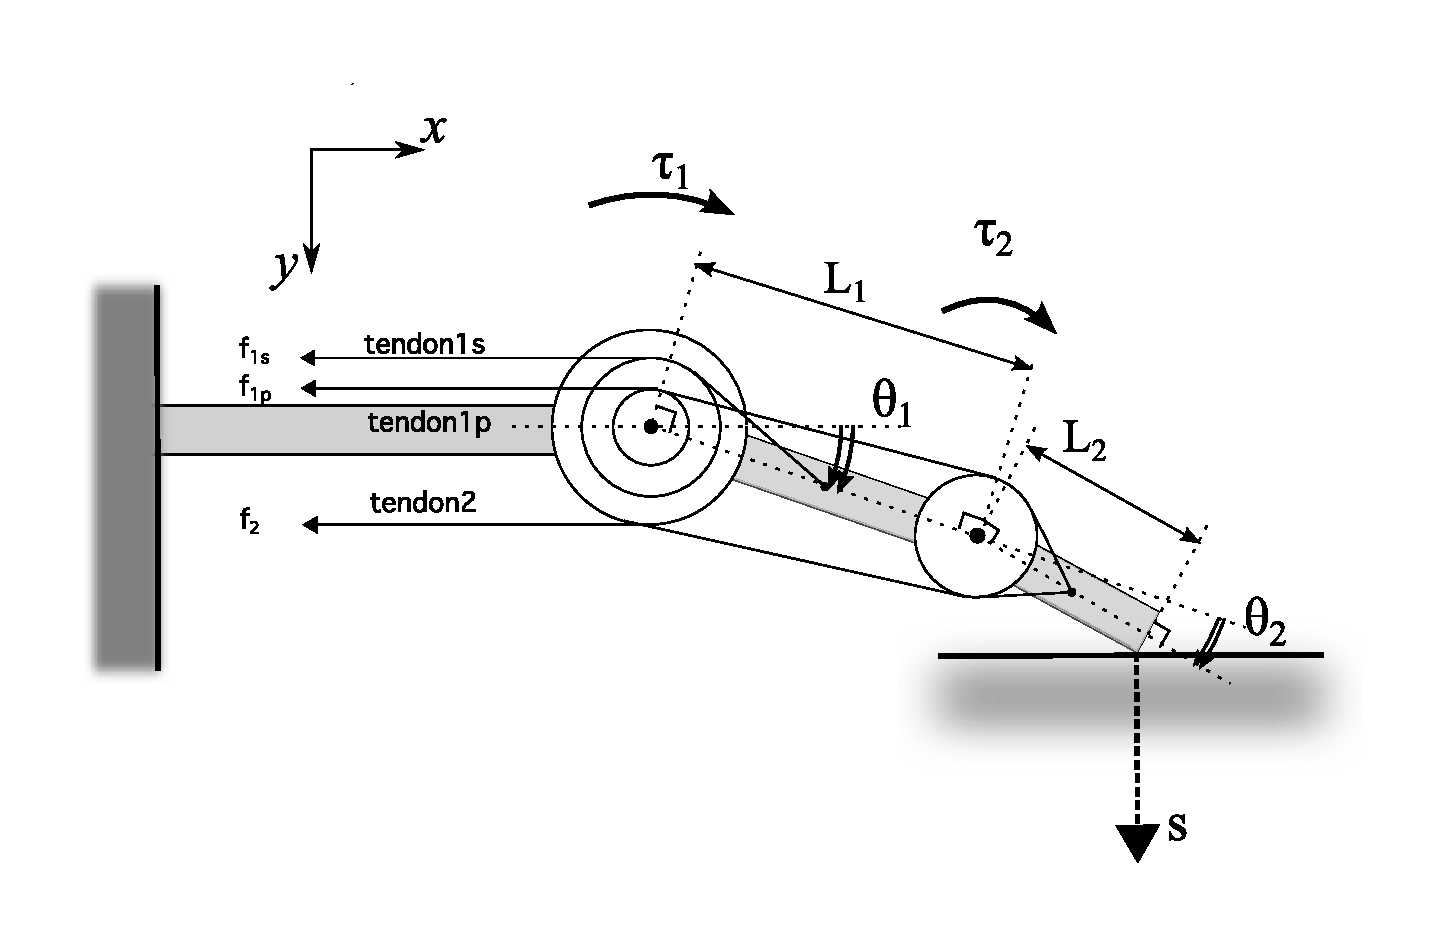
\includegraphics[width=.90\textwidth]{./figure/finger-slack.pdf}
% 																																    \caption{物体との接触}
% 																																    \label{fig:finger_slack}
% 																																   \end{figure}
																																   

% 																																   ここで,フィンガの運動を2次元に限定し,フィンガがまっすぐ伸びているときを$\theta_1,\theta_2 = 0$とし,フィンガの指先方向をx軸,矢状面上でその垂直方向をy軸とする(図\ref{fig:finger_slack}).
% 																																   このとき,静力学における$\bm{J}_r$は,

% 																																   \begin{align}
% 																																    \bm{J}_r = \begin{bmatrix}
% 																																		-(L_1\sin\theta_1 + L_2\sin(\theta_1+\theta_2)) & -L_2\sin(\theta_1+\theta_2) \\
% 																																		(L_1\cos\theta_1 + L_2\cos(\theta_1+\theta_2)) & L_2\cos(\theta_1+\theta_2)
% 																																	       \end{bmatrix},
% 																																   \end{align}

% 																																   と求まる.
% 																																   $L_1$は,関節1,2間の長さ,$L_2$は関節2と指先間の距離である.

% 																																   今,フィンガの関節が連動したまま,指先が物体に接触している状態で,指先に力を発生させることを考える.
% 																																   簡単のため,フィンガと物体の接触面には摩擦が存在しないと仮定する.
% 																																   このとき,指先にy軸方向の力しか発生していなければ,フィンガの関節は動かない.
% 																																   この,y軸方向のある力を$s$とすると,
% 																																   $\bm{s} = \begin{bmatrix}
% 																																	      0 & s
% 																																	     \end{bmatrix}^T$となる.
% 																																	     このような力を発生させる関節トルクは,式(\ref{eq:tau-s})を用いて,

% 																																	     \begin{align}
% 																																	      \bm{\tau} &= \begin{bmatrix}
% 																																			    L_1 \cos{\theta_1} + L_2 \cos(\theta_1 + \theta_2)	\\
% 																																			    L_2 \cos(\theta_1 + \theta_2)
% 																																			   \end{bmatrix} s,
% 																																	     \end{align}
																																	     
% 																																	     と求めることができる.
% 																																	     腱が独立に動かせるとき,この関節トルクを発生させる腱張力は,式(\ref{eq:f-tau-pinv})より,計算で求めることができ,

% 																																	     \begin{align}
% 																																	      \bm{f} = -\bm{A} \begin{bmatrix}
% 																																				L_1 \cos\theta_1 + L_2 \cos(\theta_1 + \theta_2)	\\
% 																																				L_2 \cos(\theta_1 + \theta_2)
% 																																			       \end{bmatrix} s + \bm{f}_b	\label{eq:slack-f}
% 																																	     \end{align}

% 																																	     と求まる.
% 																																	     この式により求まった腱張力が負になる場合,そのような腱張力は発生させることができない.
% 																																	     そのため,腱張力ベクトルの成分が負になるようなバイアス張力とフィンガが出す力$s$,関節角度が与えられたとき,負となった成分に対応する腱が緩むことになる.
% 																																	     これが腱の緩む条件となる.

% 																																	     緩む条件を満たしたトルク,バイアス張力を,分岐腱により連動している状態のフィンガの制御式に与えると,腱が緩み,関節の連動が生じなくなると考えられる.
% 																																	     ここで,1自由度のフィンガは,物体と接触すると,本来はそれ以上の動きはできないため,物体から受ける力は物体の垂直方向だけである.
% 																																	     分岐腱により関節が連動している状態のフィンガは,仮想的に1自由度とみなせるので,物体と接触しているとき,x軸方向には動かず,力が発生しない.
% 																																	     そのため,フィンガの指先には,想定したようなy軸方向の力のみが発生し,腱張力は,計算通りにかかると考えられる.
																																	     
% 																																	     % subsection tendon_slack (end)

% 																																	     % section branching_tendon (end)
	\subsection{producing} % (fold)
	\label{sub:producing}
	
we produced the robotic finger with branching tendon for developing the gripper.
finger has 2 tendons, 
finger has 2 DOFs in flexion/extension.
it is composed of 3 links and 5 pulley

	% subsection producing (end)
%  \section{2関節ロボットフィンガシステム} % (fold)
%  \label{sec:producing}
% 	実際に,グリッパを開発するため,分岐腱をもつ2関節2腱のロボットフィンガを製作した.
% 	本節では,フィンガのハードウェア仕様について言及し,その仕様に基づいて,\ref{sec:branching_tendon}節で述べたヤコビアンの具体的な値を記述する.
% 	その後,制御システムとフィンガの実際の動作について述べる.

% 	% 実際に分岐腱を持つ2関節グリッパを製作するため,その設計を行った.
% 	% 設計したグリッパの外観を図\ref{fig:finger}に示す.
% 	% 上下のフィンガの構造は,プーリの配置が鏡対称になっている以外には全く同じであり,同じフィンガを向かい合わせで固定した状態になっている.
% 	% 以下にグリッパの設計について概要を述べる.
% 	% \begin{figure}[htbp]
% 	% 	\centering
% 	% 	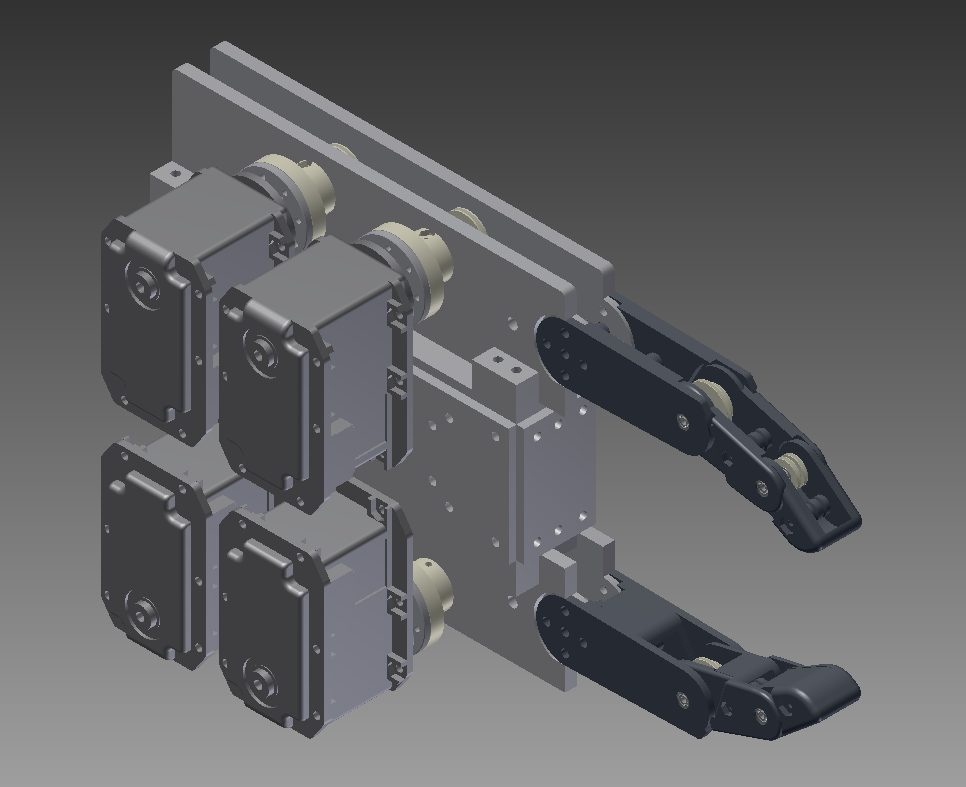
\includegraphics[width=.80\textwidth]{./figure/system4_3.png}
% 	% 		\caption{設計したグリッパ}
% 	% 		\label{fig:finger}
% 	  % \end{figure}

% 	  \subsection{各関節のモーメントアームと可動域} % (fold)
% 	  \label{sub:moment_arm}
finger movement, such as fingertip trajectory and rate of angles between coupled joints, 
can be fixed by the moment arms of each tendon. 
So, the value of moment arm is important.
Developed finger is driven by extension bifurcate tendon and flexion tendon.
% 		% フィンガの駆動に用いる腱は,屈筋1本と分岐腱を持つ伸筋1本とし,アクチュエータは1つのフィンガに対して2つとした.
% 		\ref{sub:branching_tendon}項で述べたように,フィンガの動きや関節間の連動の比率は,各腱の各関節に対するモーメントアームによって異なる.
% 		そのため,モーメントアームの決定は,フィンガの動作を決定する重要な事項である.
% 		開発するフィンガは,指先2関節を屈曲側の腱1本と伸展側の分岐腱1本で駆動する.
This arrangement of tendons is partly similar to that of man's finger.
Therefore, we decided the moment arms with reference to that of man's finger which Leijnse et al.\cite{Leijnse1995},Spoor\cite{Spoor1983} shows.
% 		この構造は,ヒトの指の先端2関節と類似する部分があり,ヒトの指における腱のモーメントアームを参考にすることが考えられる.
% 		モーメントアームの設定は,Leijnse et al.\cite{Leijnse1995},Spoor\cite{Spoor1983}の示したヒトの指におけるモーメントアームを参考にして行った.
% 		実際に採用した値を,表\ref{tab:pulley}に示す.
Tab. shows the value we use.
The moment arm $r_{t1}$ about joint1 of tendon 1 is represented as nonlinear function of PIP joint angle.
However Shirafuji et al. reproduce this with arrangement of 2 pulleys, 
in this research, we chose constant as this moment arm for siumplicity.
These moment arm are represented by the diameter of the pulleys in this design.
% 		ただし,腱1の関節1におけるモーメントアーム$r_{t1}$について,Leijnse et al.によると,このモーメントアームは,ある条件を満たすような,PIP関節の関節角度に関する非線形な関数であらわされる.
% 		Shirafuji et al.は,この非線形なモーメントアームを複数のプーリを配置することで再現しているが,本研究では,構造の簡潔化のためにこのモーメントアームは定数としている.
% 		これらのモーメントアームは各関節に腱ごとに配置されたプーリの半径によって実現されている.

The link lengths between the joints relate to fingertip force and finger trajectory.
Tab. shows this link lengths.
% 		また,各関節間の距離は,指先の軌道や指先に発生する力に関係する.
% 		フィンガの各部分の長さを表\ref{tab:system}に示す.
		
% 		\begin{table}[htbp]
% 		 \centering
% 		 \caption{プーリの半径[mm]}
% 		 \label{tab:pulley}
% 		 \begin{tabular}{|c||c|c|c|} \hline
% 		  関節 & 腱2 & 腱1p & 腱1s \\ \hline\hline
% 		  関節1 & $ r_{p1}$ & $ r_{t1}$ & $ r_{m1}$ \\
% 		  & 7 & 3 & 5 \\ \hline
% 		  関節2 & $ r_{p2}$ & $ r_{t2}$ & - \\
% 		  & 4 & 4 & - \\ \hline
% 		 \end{tabular}
% 		\end{table}

% 		\begin{table}[htbp]
% 		 \centering
% 		 \caption{フィンガの各部分の長さ[mm]}
% 		 \label{tab:system}
% 		 \begin{tabular}{|c||c|} \hline
% 		  部分 & 長さ \\ \hline\hline
% 		  指先-関節2 & 22 \\
% 		  関節2-関節1 & 30.5 \\ \hline
% 		  関節1-根元 & 45 \\
% 		  フィンガ1の根元-フィンガ2の根元 & 92 \\ \hline
% 		 \end{tabular}
% 		\end{table}

This finger's Jacobiann defined with the diameter of pulleys as follows:
% 		このフィンガにおけるヤコビアンは,式\ref{eq:J}で表されるので,表\ref{tab:pulley}を用いると,

% 		\begin{align}
% 		 \bm{J} = \begin{bmatrix}
% 			   -7 & -4 \\
% 			   3 & 4	\\ 
% 			   5 & 0
% 			  \end{bmatrix},\label{eq:J_value}
% 		\end{align}

% 		と求められる.

The rate between the changes in the joint angle vector shown by Eq.\ref{eq:rate_theta} is calculated as follows:
% 		また,実際に設計に用いた値を使って,式(\ref{eq:rate_theta})に示される関節の角速度の比を計算すると,以下のようになる.
% 		\begin{align}
% 		 \dot{\theta_1} : \dot{\theta_2} & = 1 : \frac{r_{m1}-r_{t1}}{r_{t2}} \nonumber\\
% 		 % & = 1 : \frac{r_{m1}-r_{t1}}{r_{t2}} \\ \nonumber
% 		 & = 1 : \frac{1}{2} \nonumber
% 		\end{align}

Fig. shows the fingertip trajectory of developed finger.
% 		また,このとき,フィンガを空中で動かした場合の指先の軌道は図\ref{fig:trajectory}のようになる.
% 		原点は関節1の中心で,指は始め横軸正の方向に伸びている.
		
% 		\begin{figure}[tb]
% 		 \centering
% 		 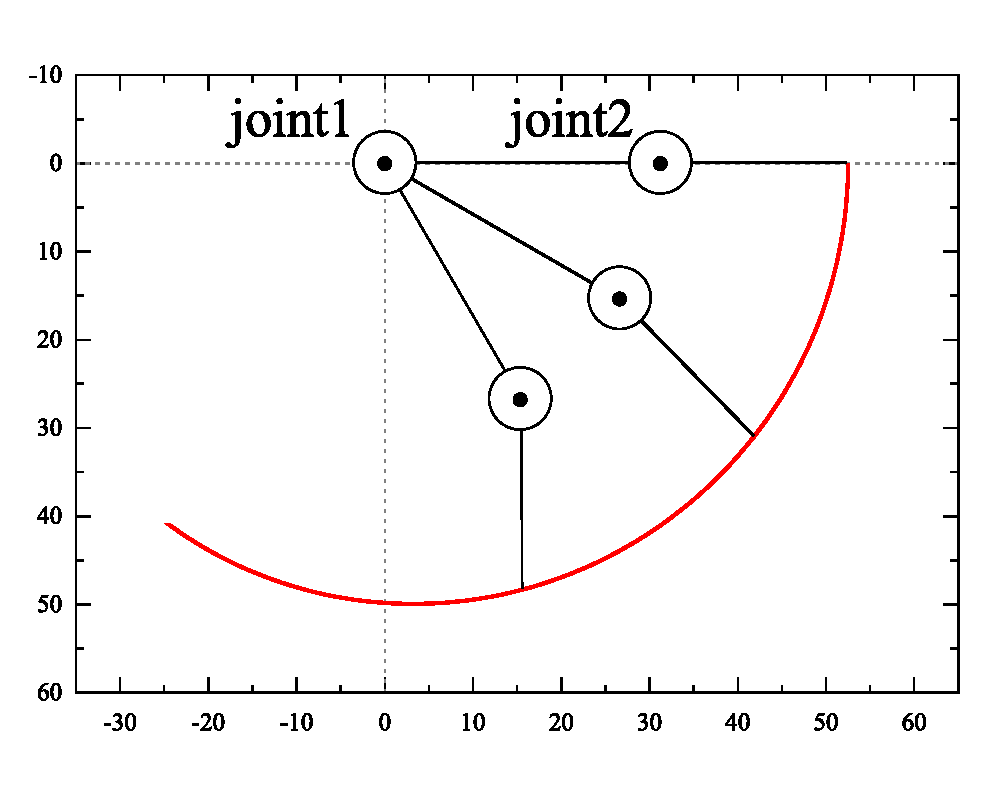
\includegraphics[width=.60\textwidth]{./figure/trajectory2.pdf}
% 		 \caption{2関節フィンガの指先の軌道(横軸,縦軸とも単位は[mm])}
% 		 \label{fig:trajectory}
% 		\end{figure}


Tab. shows the passive ranges of motion of each joints which is restricted mechanically.
% 		各関節の可動域に関しては,機械的な拘束を設けており,これによるフィンガの受動的な可動域はTable.\ref{tab:angle}の通りである.
% 		ただし,フィンガの根元から指先までが一直線となっているときを0度とし,背屈を負,底屈を正で表している.
Fig. shows max passive extension/flexion of the produced finger.
% 		実際に作成したフィンガにおける可動域は,図\ref{pic:range_motion}のようになる.
% 		ただし,外力がない場合には,図\ref{pic:range_motion2}のような伸展は起こらず,$0^{\circ}$が最大の伸展である.

% 		\begin{table}[htbp]
% 		 \centering
% 		 \caption{フィンガの可動域}
% 		 \label{tab:angle}
% 		 \begin{tabular}{|c||c|} \hline
% 		  関節2 & $0^{\circ}$ ~ $120^{\circ}$ \\ \hline
% 		  関節3 & $-40^{\circ}$ ~ $90^{\circ}$ \\ \hline
% 		 \end{tabular}
% 		\end{table}

% 		\begin{figure}[tb]
% 		 \centering
% 		 \subfigure[屈曲\label{pic:range_motion1}]{\includegraphics*[width=.45\textwidth]{./figure/JPG/range_motion3.eps}}
% 		 \subfigure[伸展\label{pic:range_motion2}]{\includegraphics*[width=.45\textwidth]{./figure/JPG/range_motion2.eps}}
% 		 \caption{フィンガの可動域}
% 		 \label{pic:range_motion}
% 		\end{figure}
		
% 		% subsection moment_arm (end)

% 		\subsection{制御システム} % (fold)
% 		\label{sub:control}
We construct control system of finger.
Fig. shows composition of control system, and Fig. shows the exterior of finger system.
Each tendons of finger is driven by servo motors(Dynamixel Mx-64R),and
tendon extension is calculated with angle measured by rotary encoders(OMRON E6A2-CW3C) connected shafts of base pulley.
And, the output pulses of encoder are counted by counter IC(NEC $\mu$ PD 4702C).
These components is controled by Arduino DUE.
Arduino orders servo motors, reads the value of counter, and calculate variables used for control of finger.

On this tendon-driven finger, tensile force and tendon extension is controled by winding tendon wire round base pulley.
Base pullry is not directly connected servo motors, but driven by torque of linear torsion spring which is put between servo motors and base pulley.
torque which spring exerts can be calculated using displacement of spring which is obtained by angles of servo and base pulley.
this torque is brought close to the target torque.
We equipped the finger with torsion springs having a spring constant of 5.17N/mm.

rotary encoders which measure angles of base pulley are directly connected shafts of base pulley.
in experiment of this developed finger, we don't have to make the finger fast movement.
so, encoder's shaft doesn't make fast rotation, recieve large radial and thrust load, we think. 

while each tendon, including branched tendon, have no slack, finger's angular position and fingertip force can be controled.
Fig. shows position control system implemnted finger.
this control is discrete system, micro computer on Arduino repeats this chain of calculation.
in figure, D reveals differentiator and S is integrator.

angular position control uses PID.
and current torque of spring is fed back to target torque calculated by position control.
restricting finger movement on horizontal plane, gravity compensation is not included in system.

when not needing position control, finger can move with only feedback control of spring torque, giving the value of joint torque which exerts target fingertip forces.

% 		フィンガを実際に動作させるため,その制御システムを製作した.
% 		システムの構成を図\ref{fig:system}に,製作したシステムの外観を図\ref{pic:finger}に示す.

% 		\begin{figure}[tb]
% 		 \centering
% 		 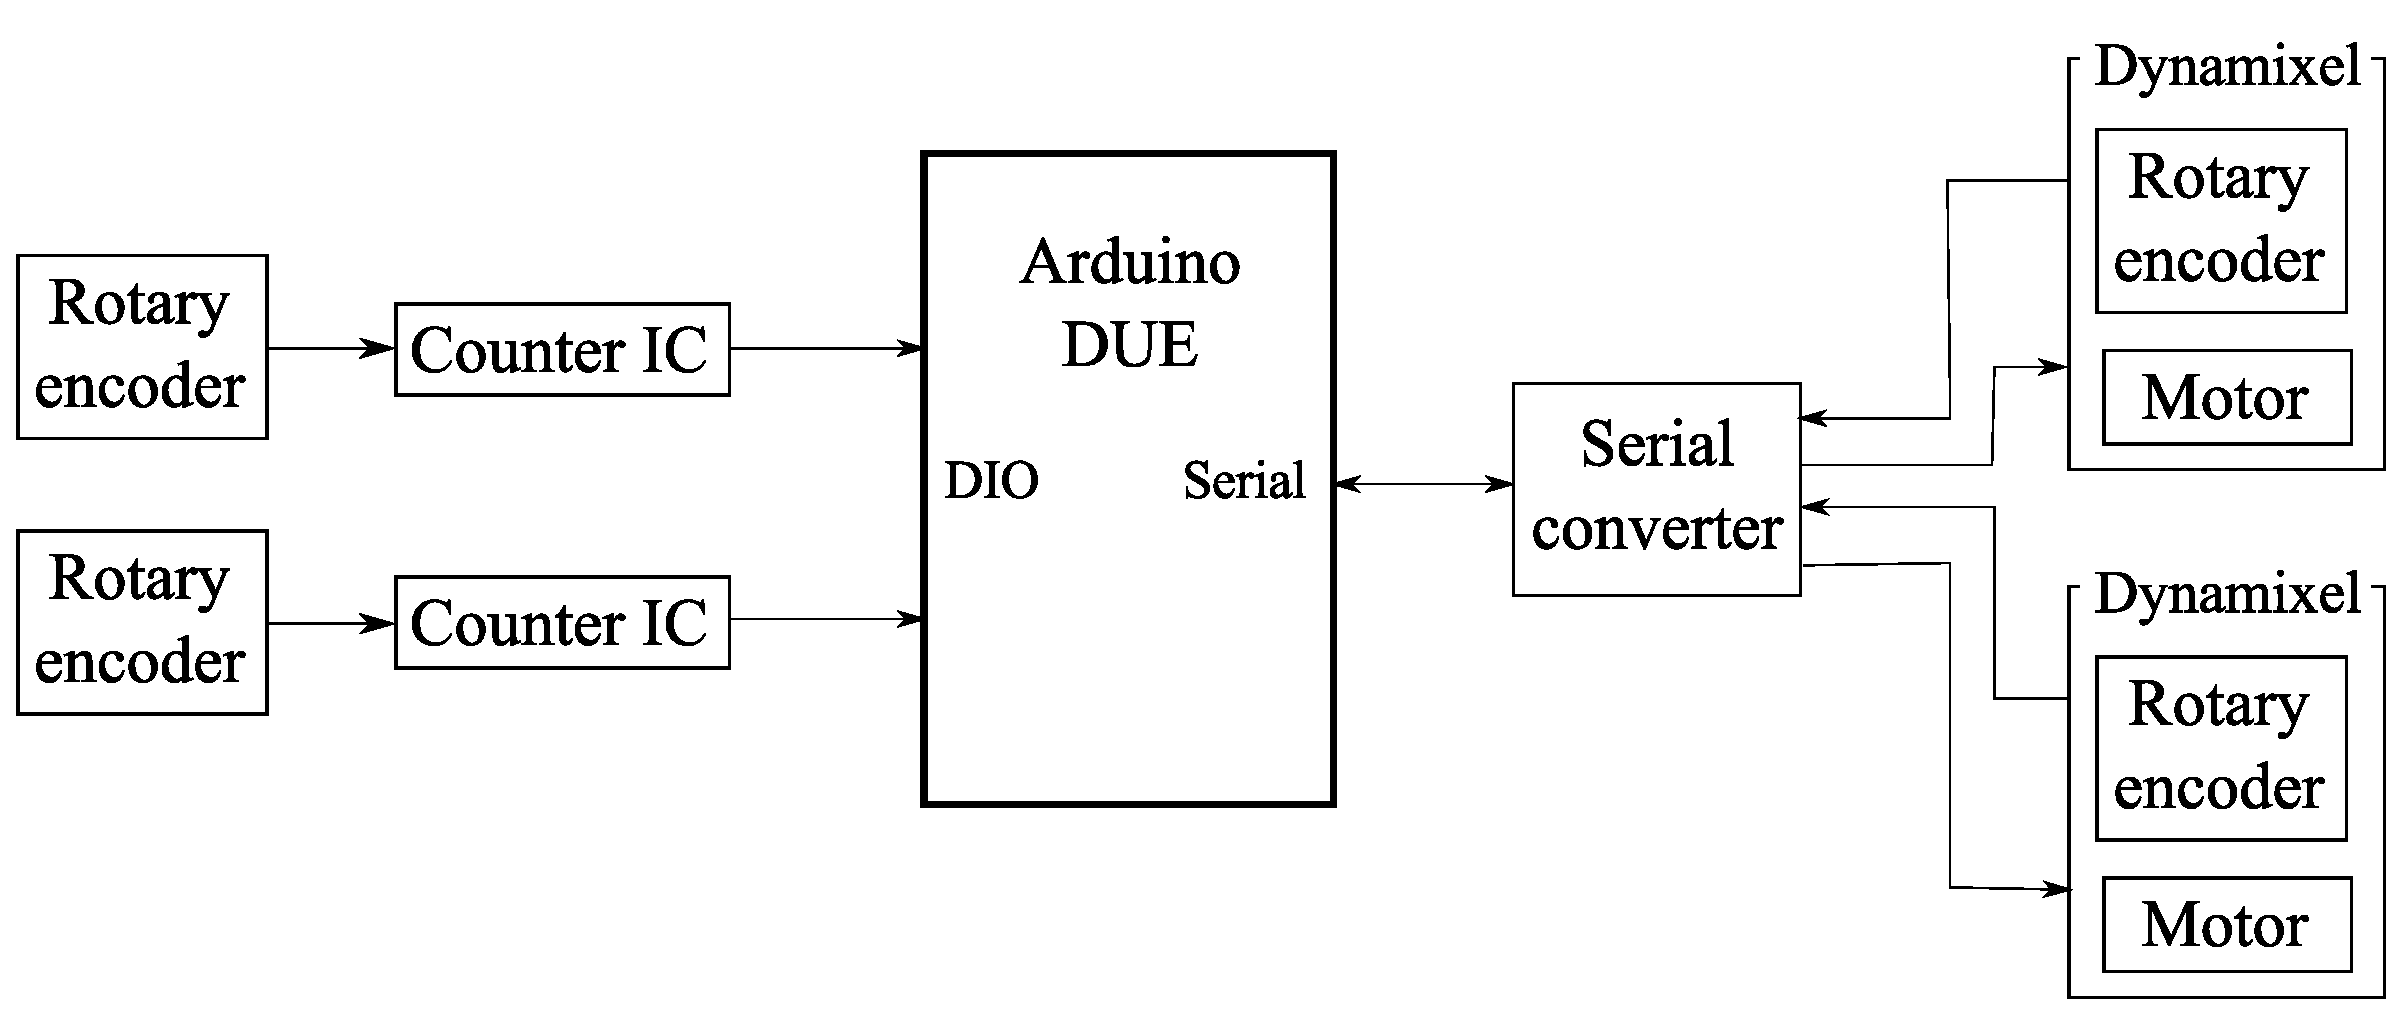
\includegraphics[width=.70\textwidth]{./figure/system.pdf}
% 		 \caption{フィンガシステム}
% 		 \label{fig:system}
% 		\end{figure}

% 		\begin{figure}[tb]
% 		 \centering
% 		 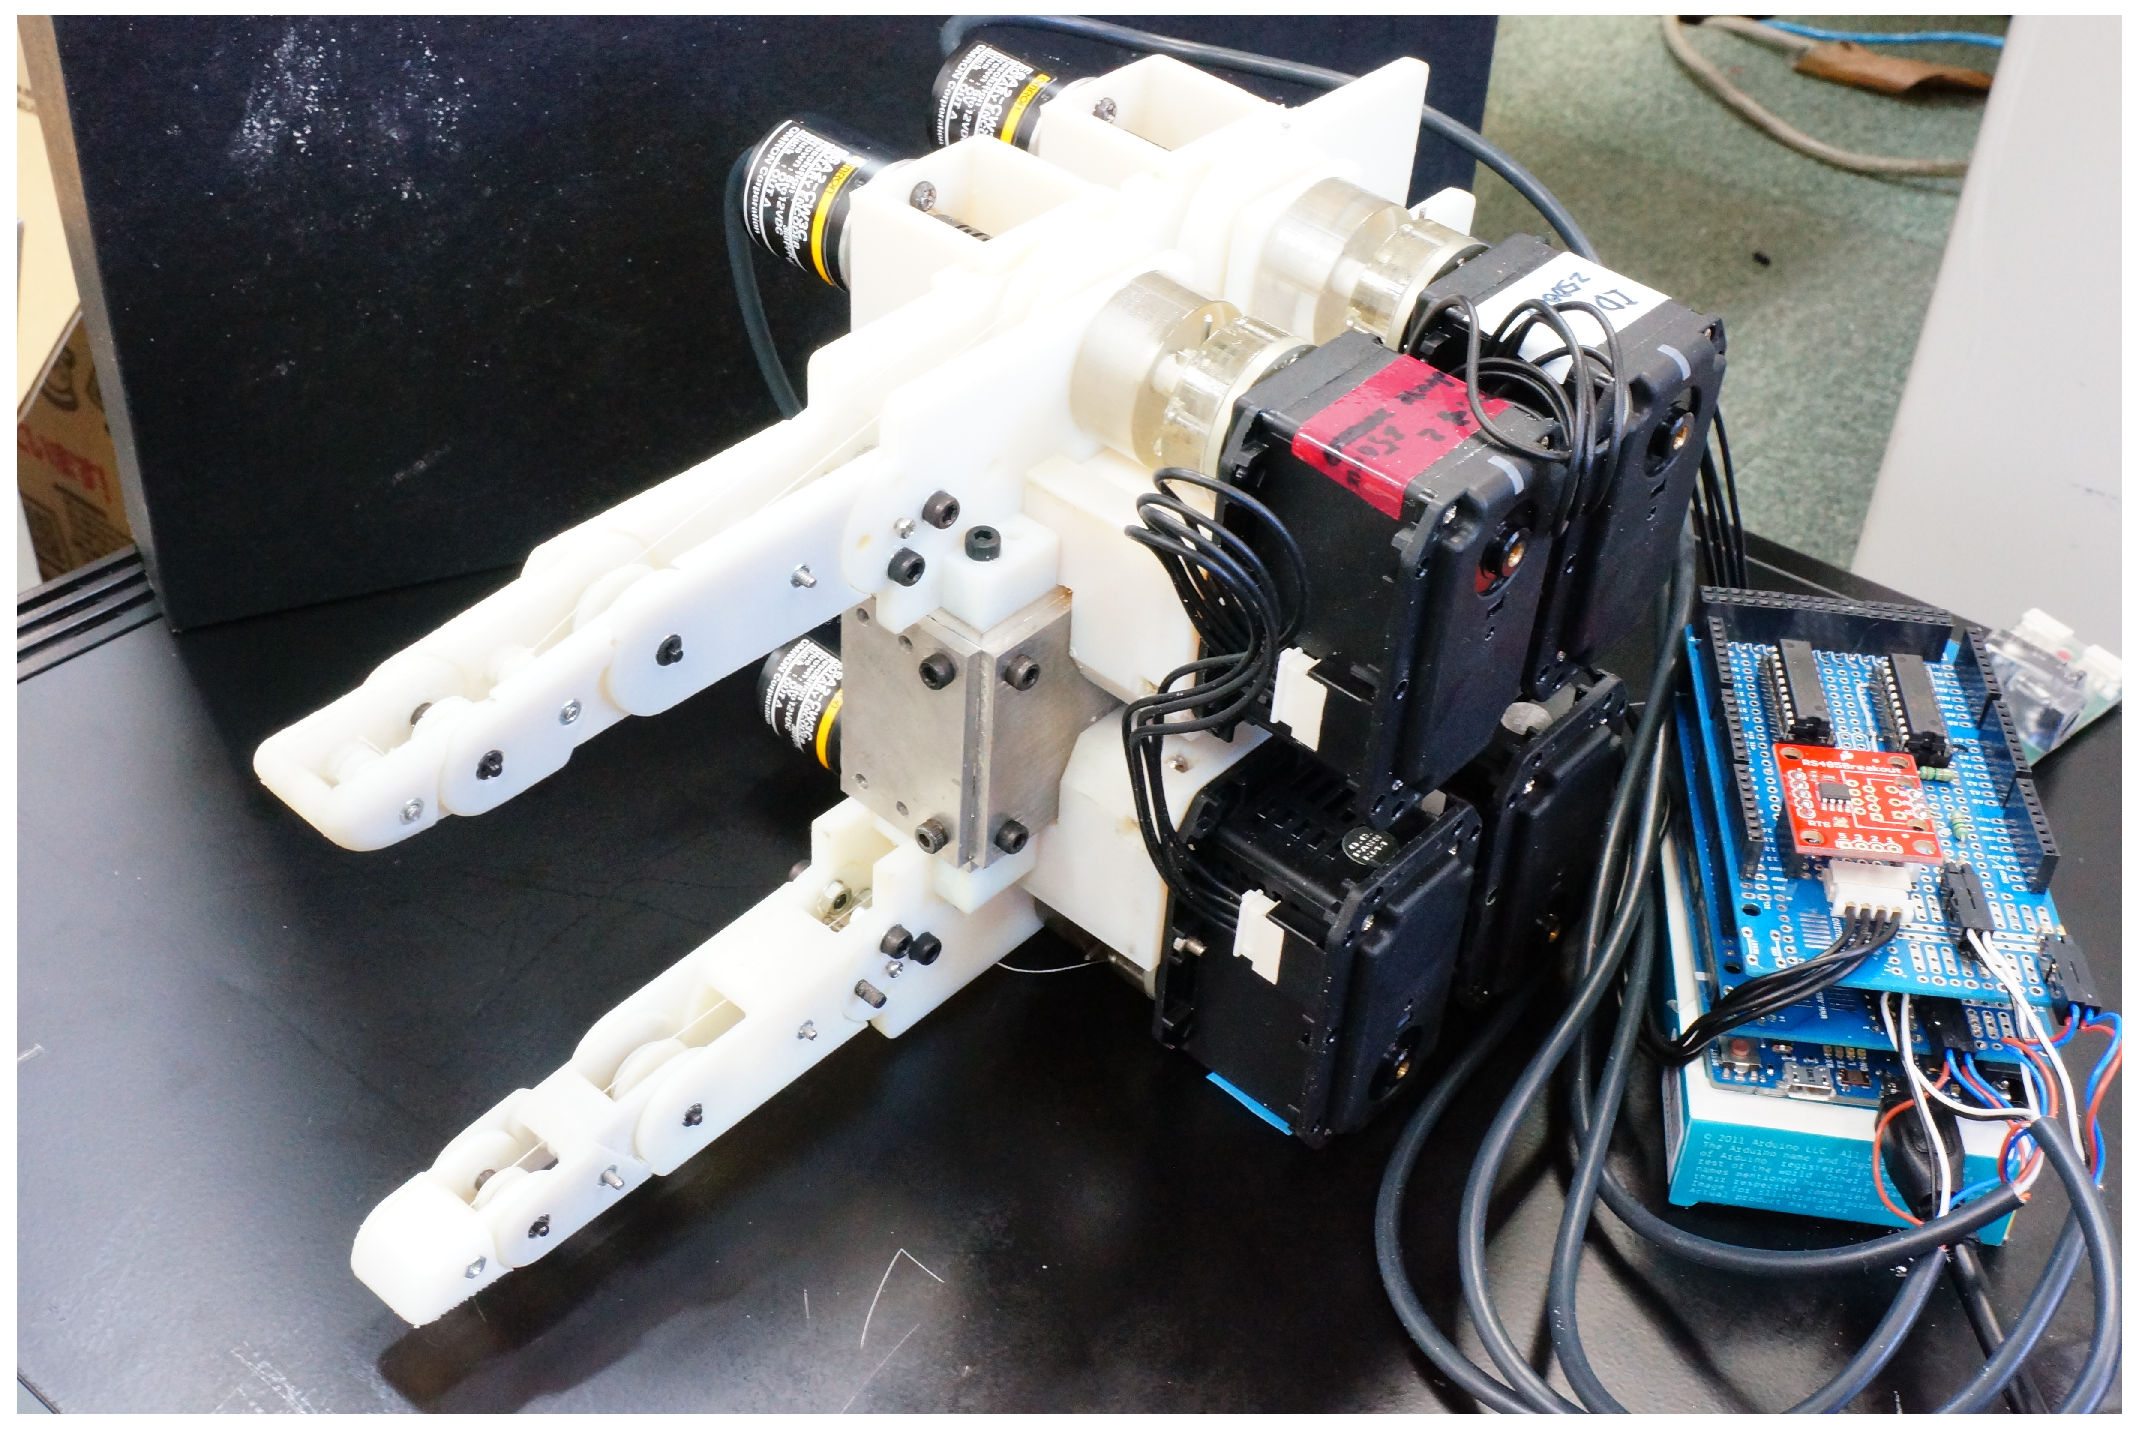
\includegraphics[width=.75\textwidth]{./figure/JPG/finger1.eps}
% 		 \caption{製作したフィンガ}
% 		 \label{pic:finger}
% 		\end{figure}

% 		フィンガには,腱を駆動するためのサーボモータと,腱の移動距離を測定するためのロータリエンコーダを,それぞれの腱に1個ずつ,計2個使用している.
% 		また,ロータリエンコーダの出力パルスをカウントするカウンタICを,エンコーダ1つにつき,1つずつ用いている.
% 		フィンガの制御に関する演算と,カウンタの読み取り,モータへの指令は,すべてマイコンボードのArduino DUEで行っている.
% 		各部品について,表\ref{tab:component}にまとめる.

% 		\begin{table}[htbp]
% 		 \centering
% 		 \caption{フィンガに搭載されているパーツ}
% 		 \label{tab:component}
% 		 \begin{tabular}{|c|c|c|}
% 		  \hline
% 		  & 型番 & 備考 \\ \hline \hline
% 		  マイコンボード & Arduino DUE & 32ビットマイコン搭載ボード,動作周波数84MHz \\ \hline
% 		  サーボモータ & Dynamixel MX-64 & 4096ビット角度センサ搭載 \\ \hline
% 		  ロータリエンコーダ & OMRON E6A2-CW3C & インクリメンタル方式,2相,360P/R \\ \hline
% 		  カウンタIC & NEC $\mu$PD4702C & 8ビット・アップ・ダウン・カウンタ \\ \hline
% 		 \end{tabular}
% 		\end{table}

% 		腱駆動のフィンガは,腱の巻き取り量を調整することで,腱張力や腱の移動速度を制御する.
% 		開発したフィンガにおいては,腱に発生する張力を制御するため,腱をモータで直接巻き取るのではなく,ねじりばねを用いることで,力を伝達している.
% 		具体的には,腱を駆動するプーリと,モータの間にねじりばねをはさみ(図\ref{fig:spring}),モータを位置制御することでプーリに発生するトルクを制御する.
% 		ばねに発生しているトルクは,プーリとモータの位置から求まるばねの変位によって計算することができ,このトルクが目標トルクに達するように制御を行う.
% 		今回使用したばねは,ばね定数5.17[N mm/deg],許容変位値30[deg]である.

% 		ロータリエンコーダの取り付けは,簡単のため,駆動軸と直結することにした(図\ref{fig:spring2}).
% 		開発したフィンガでは,駆動軸が高速に回転することはなく,ラジアル方向,スラスト方向ともに,軸に大きな力がかかることはないと判断した.

% 		\begin{figure}[tb]
% 		 \centering
% 		 \subfigure[ねじりばね\label{fig:spring1}]{\includegraphics*[width=.45\textwidth]{./figure/JPG/spring1.eps}}
% 		 \subfigure[駆動軸周り\label{fig:spring2}]{\includegraphics*[width=.45\textwidth]{./figure/JPG/spring2.eps}}
% 		 \caption{駆動部分}
% 		 \label{fig:spring}
% 		\end{figure}

% 		フィンガは,分岐腱に緩みがないとき,位置制御,もしくは指先に発生する力の制御を行える.
% 		位置制御するときは,図\ref{fig:control}に示すように制御を行う.

% 		\begin{figure}[tb]
% 		 \centering
% 		 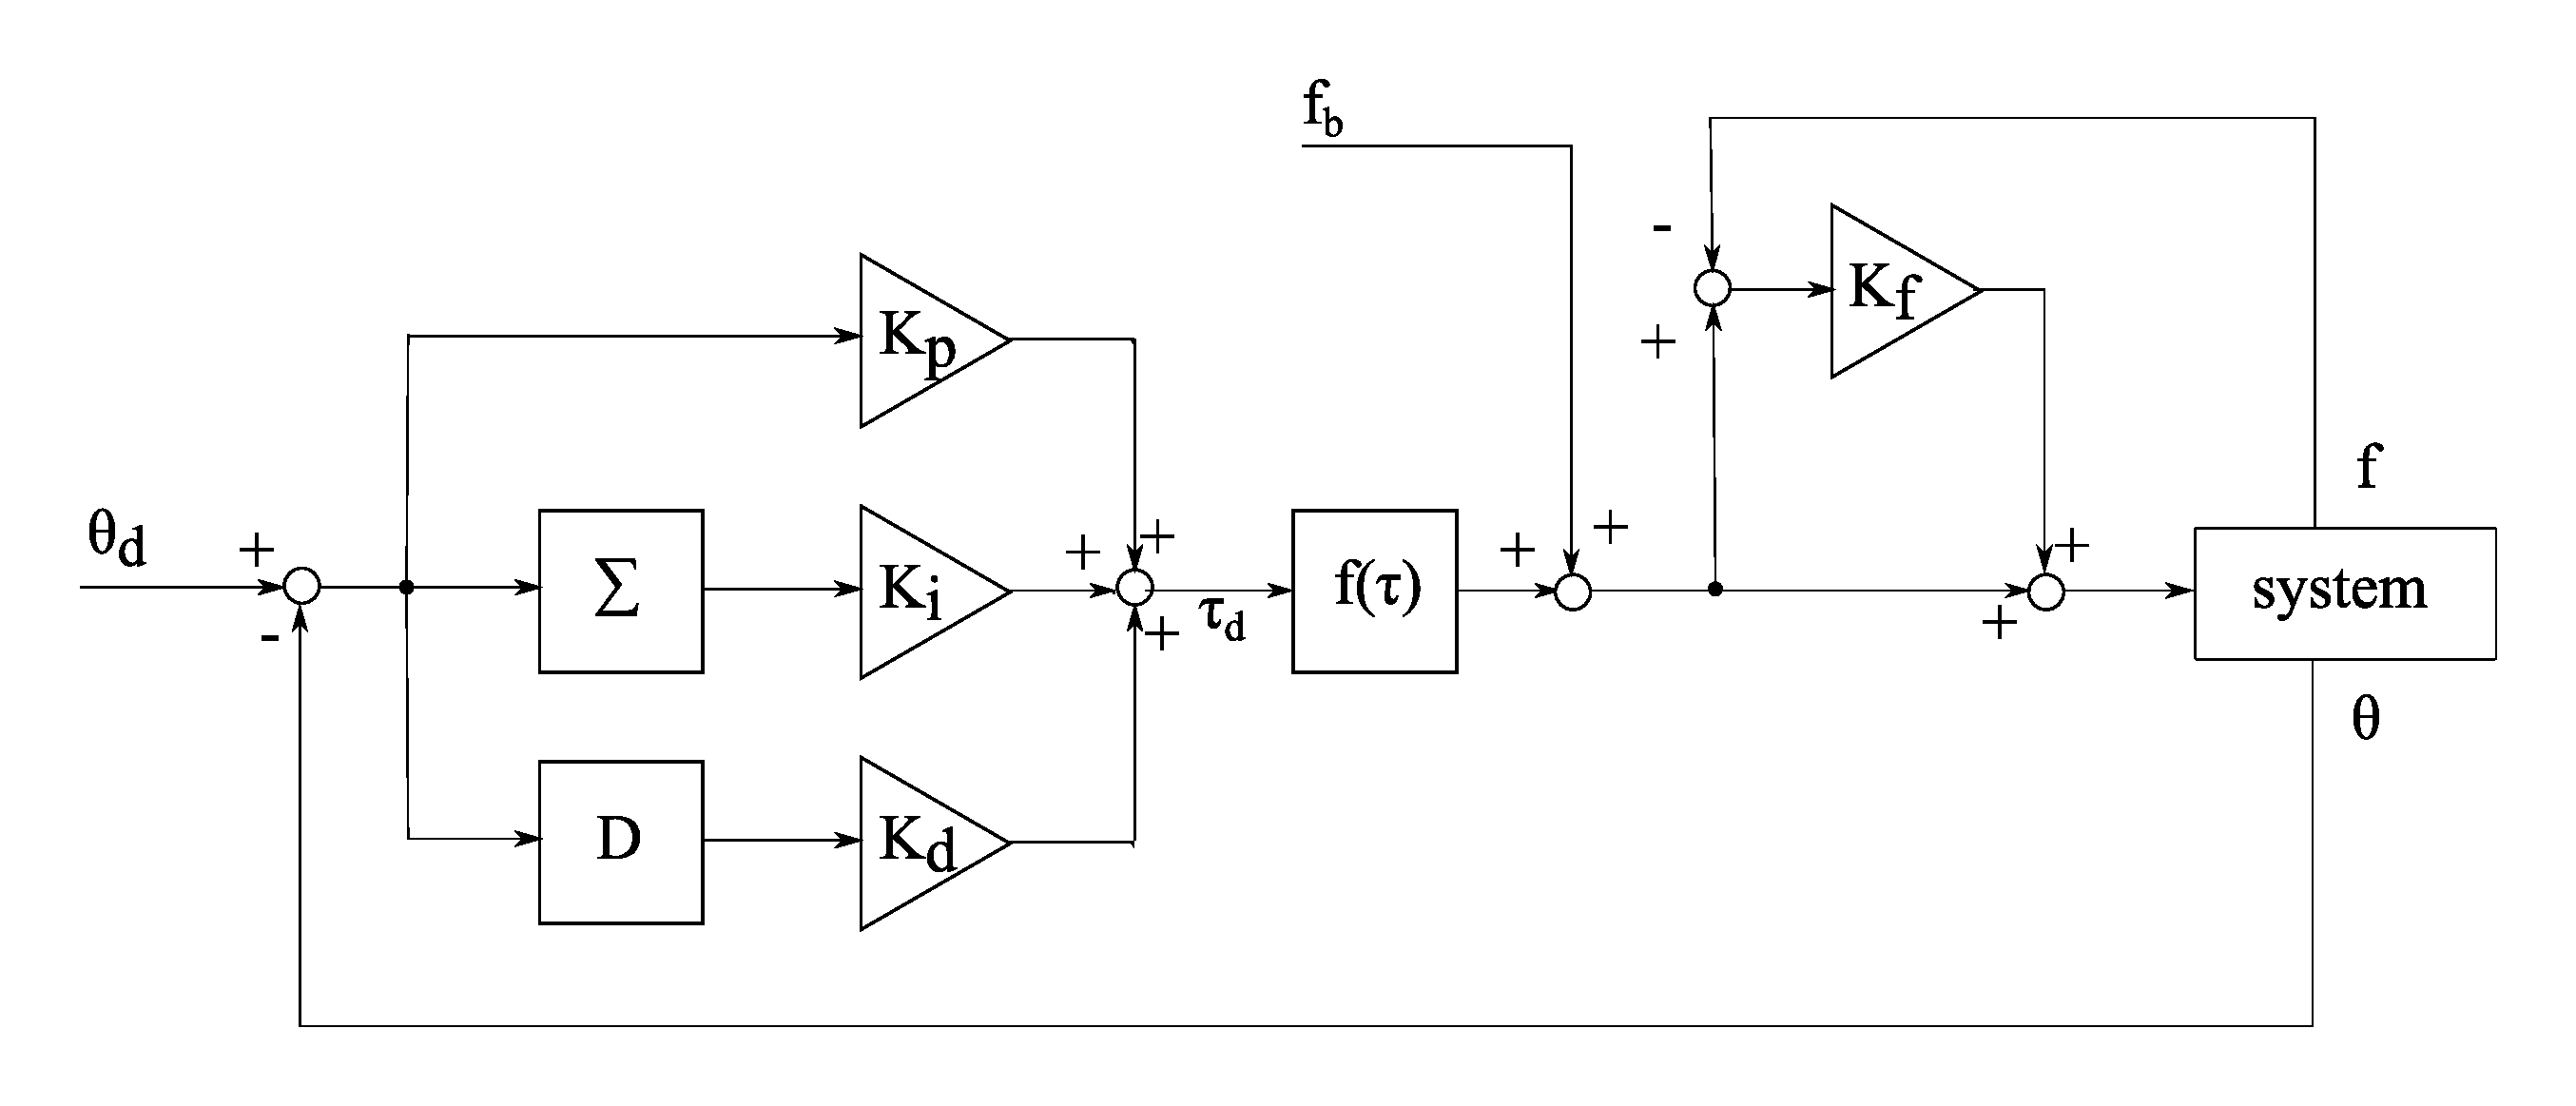
\includegraphics[width=\textwidth]{./figure/control.pdf}
% 		 \caption{位置制御のブロック線図}
% 		 \label{fig:control}
% 		\end{figure}

% 		この制御は,離散システムであり,マイコンでこの一連の計算を繰り返し行っている.
% 		図中の$D$は微分器を,$\Sigma$は積分器を表す.

% 		位置制御は,目標値とのずれに対してPID制御を行っている.
% 		また,PID制御の結果の目標トルクに対して,実際に駆動軸に発生しているトルクとのずれをフィードバックしている.
% 		フィンガは,水平面内で動作することとし,重力補償は行っていない.

% 		物体に接触させて,力をかけるときなど,位置制御を行わないときは,指先に出したい力を発生させる関節トルクを指令値として与え,関節トルクのフィードバックのみで制御を行う.


bias force

Fig. shows  when controling angles 
% 		以上のようなシステムでフィンガを動作させる.
% 		実際に,関節1の角度が0度の位置から40度の位置まで位置制御を行ったときの,目標角度値に対する,腱の変位から計算される関節1の角度のグラフを図\ref{fig:angle_tracking}に示す.
% 		また,関節1の角度が0度の位置から40度の位置まで位置制御を行ったときの,フィンガの動きを図\ref{pic:angle_tracking}に示す.

% 		\begin{figure}[tb]
% 		 \centering
% 		 \subfigure[0度から40度への移動\label{fig:angle}]{\includegraphics*[width=.90\textwidth]{./figure/plot/0208_3_0-20.pdf}}\\
% 		 \subfigure[40度から20度への移動\label{fig:angle2}]{\includegraphics*[width=.90\textwidth]{./figure/plot/0208_4_20-10.pdf}}\\
% 		 % \subfigure[0119\_10-40\label{fig:angle3}]{\includegraphics*[width=.85\textwidth]{./figure/plot/0119_v13_10-40.pdf}}%場所埋め,いらなかったら削除
% 		 \caption{位置制御時の関節1の目標角度と実際の角度の推移}
% 		 \label{fig:angle_tracking}
% 		\end{figure}

% 		\begin{figure}[tbh]
% 		 \centering
% 		 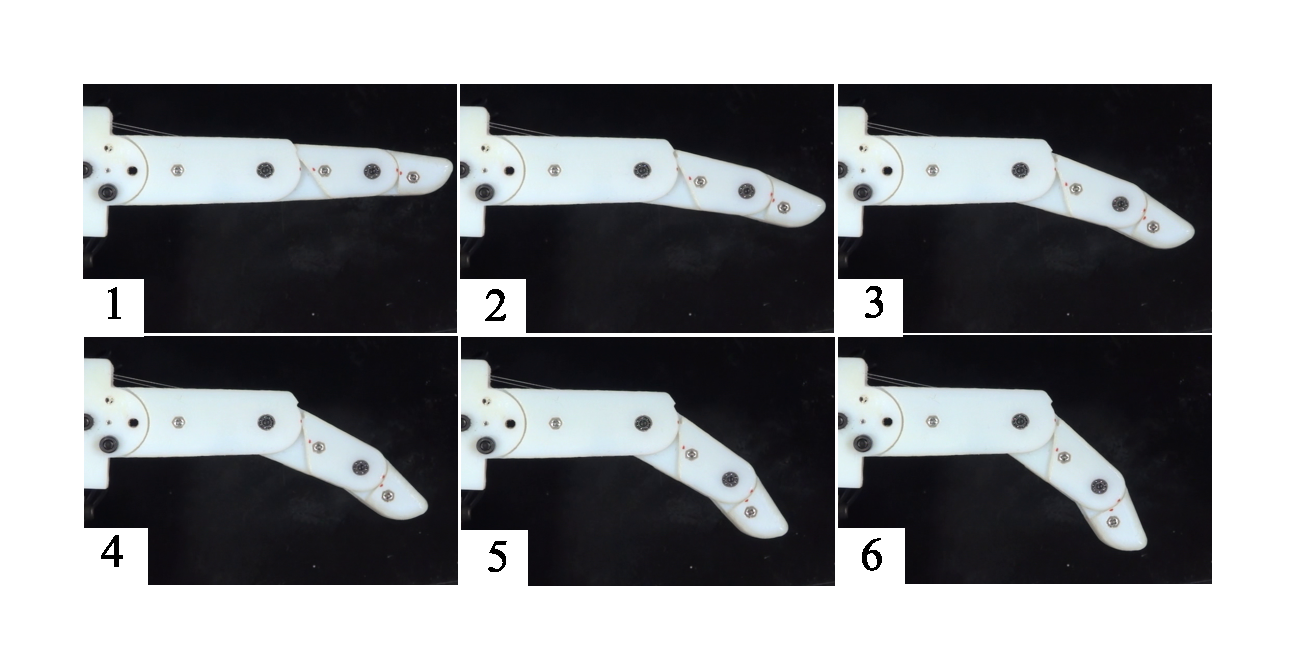
\includegraphics[width=\textwidth]{./figure/frame0208.pdf}
% 		 \caption{位置制御時のフィンガの動き}
% 		 \label{pic:angle_tracking}
% 		\end{figure}

Tab. shows Gain constant when position controling.
% 		このときの位置制御における各ゲインは,表\ref{tab:gain}の通りである.

% 		\begin{table}[htbp]
% 		 \centering
% 		 \caption{位置制御におけるゲイン}
% 		 \label{tab:gain}
% 		 \begin{tabular}{|c|c|}
% 		  \hline
% 		  $K_p$ & 0.05\\ \hline
% 		  $K_i$ & 0.01\\ \hline
% 		  $K_d$ & 0.001\\ \hline
% 		  $K_f$ & 0.1\\ \hline
% 		 \end{tabular}
% 		\end{table}

We look up delay of initial response in Fig.
This can be caused by rotational friction of joint.
Though finger's joints 
not shaft but 
In this time, we didn't sufficiently configulate each gain constant because position control is not main focus in this research.
If we had to improve responsibility, we had better configure gain.
% 		グラフからは,フィンガの初動が遅れていることが読み取れる.
% 		これは,関節の回転方向に生じる摩擦力が大きいためだと考えられる.
% 		フィンガの関節には,ボールベアリングが入っており回転軸における摩擦は十分に小さい.
% 		しかし,関節において,フィンガの外装同士が干渉していることが考えられる.
% 		% しかし,軸が,地面と平行になった状態で動作させているため,関節において,.
% 		これを防止する十分なクリアランスが設定できていなかったため,摩擦が大きくなってしまっていると考えられる.

% 		また,目標値への角度の収束が十分に早いとは言えない.
% 		さらに,目標角度が一定のときの外乱に対しても,すぐに抵抗する力が弱く,目標角度への移動にはかなり時間がかかる.
% 		今回は,動作確認のために位置制御を行ったので,PID制御におけるゲインを十分に調整していなかった.
% 		しっかりとゲイン調整を行えば,時間に対する応答性は良くなることが予想される.
		
% 		% (位置制御時の腱張力の割合,それにともなう動きなどについて追加する.また,ヤコビアンの値から,仮想自由度での制御に用いている式を示しておく?)
% 		% subsection control (end)

% 		% section producing (end)

%  \section{開発したフィンガによるグリッパ} % (fold)
%  \label{sec:gripper}
% 	開発したフィンガを2本組み合わせることで,グリッパとして利用することができると考えられる.
% 	その外観は,図\ref{pic:finger}に示した通りである.
% 	グリッパとしての動きのイメージを図\ref{fig:gripper}に示す.
% 	まず,物体に接触するまでは,図\ref{fig:gripper_coupled}に示すように,関節が連動した状態で動かす.
% 	このとき,関節は連動しているので,1自由度のグリッパのように,物体に決まった軌道でアプローチすることになる.
% 	この状態から,バイアス張力を減らしていく,もしくは,指先の力を強めていくと,図\ref{fig:gripper_uncoupled1}のように腱が緩み,形態が変化するようなグリッパとして用いることができるのではないかと考えられる.

% 	\begin{figure}[tb]
% 	 \centering
% 	 \subfigure[連動している状態\label{fig:gripper_coupled}]{\includegraphics*[width=.48\textwidth]{./figure/gripper.pdf}}
% 	 \subfigure[腱1sが緩んだ状態\label{fig:gripper_uncoupled1}]{\includegraphics*[width=.48\textwidth]{./figure/gripperuncoupled1.pdf}}
% 	 \caption{2関節フィンガによるグリッパの模式図}
% 	 \label{fig:gripper}
% 	\end{figure}

\section{verification of tendon slack} % (fold)
\label{sec:verification}


% \chapter{2関節フィンガにおける分岐腱の緩み条件の検証} % (fold)
% \label{cha:verification}
Tendon of developed robotic finger can get slack of one of the branching tendon, 
depending on the condition of both bias tensile force of all tendons and fingertip force exerted.
We verified whether finger in real environment move along the theory which we shows previous section with developed finger.
% 	\ref{sub:tendon_slack}項で述べたように,開発したロボットフィンガでは,フィンガが指先に発生する力と腱のバイアス張力の条件によって,腱に緩みが生じる.
% 	計算により求めたこの条件が,実際の状況に即しているかどうか,実機により検証を行った.
% 	本章では,検証実験の手順と結果について述べる.


% 	\section{緩み条件検証の手順} % (fold)
% 	\label{sec:slack_experiment}
% 		\ref{sub:tendon_slack}項で計算されたように,分岐腱の緩み条件は,フィンガの角度や指先の力によって決まる.
% 		ここでは,開発したフィンガにおける緩み条件の具体的な値と,実験の手順について述べる.
% 		% 実験設定について述べる.
% 		% 使った板,角度,力の大きさ,フィンガの動かし方など.
% 		% 図があればいいか.
% 		% 動いている写真?
% 		% バイアスレートの取り方

% 		% \subsection{フィンガ先端の形状} % (fold)
% 		% \label{sub:fingertip_attatchment}
% 		% 	開発したフィンガの指先パーツの先端は,曲面で構成されており,物体との接触点が分かりにくく,緩み条件の計算が難しくなってしまう.
% 		% 	そのため,指先パーツを覆う新たなパーツを設計し,装着して実験を行うこととした.
% 		% 	指先に装着した様子を,図\ref{fig:fingertip_attachment}に示す.
% 		% 	フィンガを伸ばしたときに,物体との接触点が,関節を結んだ直線上に乗るようにした.
% 		% 	このパーツを装着した場合の,関節2から指先までの距離は,37.5[mm]である.
			
% 		% 	\begin{figure}[tbhp]
% 		% 		\centering
% 		% 		\subfigure[\label{fig:fingertip1}]{\includegraphics*[width=.40\textwidth]{./figure/JPG/fingertip1.eps}}
% 		% 		\subfigure[\label{fig:fingertip2}]{\includegraphics*[width=.40\textwidth]{./figure/JPG/fingertip2.eps}}
% 		% 		\caption{指先追加パーツ}
% 		% 		\label{fig:fingertip_attachment}
% 		% 	\end{figure}

% 		% 	このように,フィンガの指先には新たなパーツを取り付けることができるようになっており,柔らかい素材で皮膚を取り付けるといったことも,ある程度可能である.

% 		% % subsection fingertip_attatchment (end)

% 		\subsection{フィンガにおける緩み条件} % (fold)
% 		\label{sub:valiables_of_slack}
	In order to make tendons of the finger slacken, either value of tensile force of tendon 1s or 1p which is calculated by Eq.\ref{eq:slack-f} have to become negative.
	Because the tendon Jacobian about developed finger is represented as Eq.\ref{eq:J_value}, 
	$\bm{A}$, $\bm{f}_b$ in Eq.\ref{eq:f-tau-pinv} is defined as follows:

% 			腱が緩む条件は,式(\ref{eq:slack-f})で計算される腱張力ベクトルの成分のうち,腱1p,1sの腱張力どちらかが負になることである.

% 			本研究で開発したフィンガにおいて,腱ヤコビアン$\bm{J}$は式(\ref{eq:J_value})のように与えられるので,これを用いて,式(\ref{eq:f-tau-pinv})における$\bm{A}$,$\bm{f}_b$を計算すると,

 			\begin{align}
				\bm{A} = \begin{bmatrix}
					-0.0606 & -0.0492	\\
					-0.0606 & 0.2008	\\
					0.1515 & -0.1894
				\end{bmatrix},	
				\bm{f}_b = \begin{bmatrix}
					1 \\
					1 \\
					0.8
				\end{bmatrix}f_b, 
			\end{align}

	where $f_b$ is the bias tensili force variable.
	$f_b$ can be described ...
% 			となる.
% 			ここで,式(\ref{eq:f-tau-pinv})において,$\bm{\xi} = \xi\begin{bmatrix}1 & 1 & 1\end{bmatrix}^T$とし,さらに,$\bm{f}_b$の腱2に対するバイアス張力が$f_b$となるように,係数$\xi$を調整したものを,$f_b$とおいている.

	When coupling of two joints, using $\theta_1=2\theta_2$, $\bm{f}$ is described from Eq.\ref{eq:slack-f} as follows:
% 			これより,式(\ref{eq:slack-f})において,$\bm{f}$を求めると,

% 			\begin{align}
% 				\bm{f} = \begin{bmatrix}
% 					f_2		\\
% 					f_{1p}	\\
% 					f_{1s}
% 				\end{bmatrix} = \begin{bmatrix}
% 					0.0606L_1\cos\theta_1+0.1098L_2\cos(\theta_1+\theta_2)	\\
% 					0.0606L_1\cos\theta_1-0.1402L_2\cos(\theta_1+\theta_2)	\\
% 					-0.1515L_1\cos\theta_1+0.0387L_2\cos(\theta_1+\theta_2)
% 				\end{bmatrix}s
% 				+\begin{bmatrix}
% 					1 \\
% 					1 \\
% 					0.8
% 				\end{bmatrix}f_b,
% 			\end{align}

% 			となる.
% 			さらに,関節が連動しているとき,$\theta_1 = 2\theta_2$なので,

% 			\begin{align}
% 				\bm{f} = \begin{bmatrix}
% 					f_2		\\
% 					f_{1p}	\\
% 					f_{1s}
% 				\end{bmatrix} = \begin{bmatrix}
% 					0.0606L_1\cos2\theta_2+0.1098L_2\cos3\theta_2	\\
% 					0.0606L_1\cos2\theta_2-0.1402L_2\cos3\theta_2	\\
% 					-0.1515L_1\cos2\theta_2+0.0387L_2\cos3\theta_2
% 				\end{bmatrix}s
% 				+\begin{bmatrix}
% 					1 \\
% 					1 \\
% 					0.8
% 				\end{bmatrix}f_b,\label{eq:independent-f}
% 			\end{align}

% 			となる.
% 			ここで,腱張力が負にならないように調整できる変数は3つ存在する.
% 			1つは,フィンガが指先に出す物体に対して垂直な方向の力の大きさ$f$である.
% 			2つ目は,物体に接触したときの関節2の角度$\theta_2$である.
% 			最後は,腱のバイアス張力$\bm{f}_b$の大きさである.
	When $f$ and $\theta_2$ is fixed, the value of $f_b$ which make $f_{1p}$ or $f_{1s}$ to zero is calculated.
	When $f_b$ fall short of this value, tensile force of one of the branch get minus and that branch slacken.
	Fig.\ref{fig:slack} shows this value of $f_b$.
	Fig.\ref{fig:slack-angle}...
% 			ここでは,$f$と$\theta_2$をそれぞれ固定したときに,$f_{1p}$,もしくは$f_{1s}$がちょうど$0$になる$f_b$の値を,分岐腱の緩みの条件として考え,図\ref{fig:slack}に示す.
% 			図\ref{fig:slack-angle}は,$f=0.6$としたときの,角度$\theta_2$に対して,$f_{1p}$,$f_{1s}$がちょうど$0$になる$f_b$の値ををれぞれグラフにしたものである.
% 			グラフの横軸は関節2の角度であり,フィンガが最大に伸展している状態の$\theta_2=0^{\circ}$から,フィンガの指先が物体に対して垂直になる,$\theta_2=30^{\circ}$までを範囲としている.
% 			図\ref{fig:slack-force}は,$\theta_2=15^{\circ}$としたときの,$s$に対して,$f_{1p}$,$f_{1s}$がちょうど$0$になる$f_b$の値ををれぞれグラフにしたものである.
% 			グラフの横軸は,フィンガが指先に発生させる力であり,フィンガに使用したねじりばねの最大トルクを考慮して$s=2$までを範囲としている.

% 			\begin{figure}[tbhp]
% 				\centering
% 				\subfigure[$f=0.6$のときの,角度に対する緩み条件\label{fig:slack-angle}]{\includegraphics*[width=.49\textwidth]{./figure/plot/threshold_angle.pdf}}
% 				\subfigure[$\theta_2=15^{\circ}$のときの,指先に発生する力に対する緩み条件\label{fig:slack-force}]{\includegraphics*[width=.49\textwidth]{./figure/plot/threshold_force.pdf}}
% 				\caption{緩み条件}
% 				\label{fig:slack}
% 			\end{figure}

% 			ここで,開発したフィンガの指先に追加パーツをつけたため,$L_1=30.5,L_2=37.5$として計算した.

	As figure shown, on the developed finger, the value of $f_b$ which make $f_{1s}$ to zero is larger than that of $f_{1p}$ in any $\theta_2$, $s$.
	Therefore, $f_{1s}$ fall to zero and tendon 1s loosen before $f_{1p}$ do, while gradually lowering $f_b$.
% 			グラフに示した値を下回る$f_b$をバイアス張力としてかけてフィンガを動作させると,対応する腱の張力は負になるため,腱が緩む.
% 			グラフから分かるように,開発したフィンガでは,グラフに示されている範囲において,いかなる$\theta_2$,$s$の値においても,腱1pよりも腱1sの方が,張力が0になる$f_b$の値が大きい.
% 			したがって,$f_b$を十分に大きい値から徐々に下げていくと,腱1sの張力が先に0となり,腱が緩むことになる.

	In order to make tendon 1p slack, 
% 			この条件には,計算の過程から分かるように,フィンガの腱ヤコビアンが関係する.
% 			また,腱ヤコビアンの成分は,腱のモーメントアームになっているので,今回開発したフィンガとは違い,腱1pを先に緩ませようと思うと,モーメントアームを変更する必要がある.
% 			このようなモーメントアームの一例としては,表\ref{tab:slack_momentarm}のような組み合わせがある.

% 			\begin{table}
% 				\centering
% 				\caption{異なる緩み状態を実現するモーメントアームの一例}
% 				\label{tab:slack_momentarm}
% 				\begin{tabular}{|c||c|c|c|} \hline
% 					関節 & 腱2 & 腱1p & 腱1s \\ \hline\hline
% 					関節1 & $ r_{p1}$ & $ r_{t1}$ & $ r_{m1}$ \\
% 					 & 15 & 3 & 5 \\ \hline
% 					関節2 & $ r_{p2}$ & $ r_{t2}$ & - \\
% 					 & 1 & 4 & - \\ \hline
% 				\end{tabular}
% 			\end{table}

% 			モーメントアームは,フィンガの関節に組み込まれているプーリによって実現しているため,変更には,新たなプーリを製作する必要がある.
			
% 			今回は,新たなプーリを作り,緩みを再現することはしないが,このように,モーメントアームの変更により,緩む腱を選ぶことができる.

% 			% 余った画像貼る?
% 			% \begin{figure}[htbp]
% 			% 	\centering
% 			% 	\subfigure[\label{fig:slack-force1}]{\includegraphics*[width=.48\textwidth]{./figure/slack.png}}
% 			% 	% \subfigure[\label{fig:slack-force2}]{\includegraphics*[width=.48\textwidth]{./figure/slack.png}}
% 			% 	\caption{指先に発生させる力に対する緩み条件}
% 			% 	\label{fig:slack-force}
% 			% \end{figure}

% 		% subsection valiables_of_slack (end)

% 		\subsection{実験方法} % (fold)
% 		\label{sub:process_of_experiment}
% 			前節で述べた,開発したフィンガにおける分岐腱の緩み条件が,実際の動きとどの程度一致するか,検証のため実験を行った.
% 			実験の様子を,図\ref{pic:experiment}に示す.
			
% 			\begin{figure}[tbhp]
% 				\centering
% 				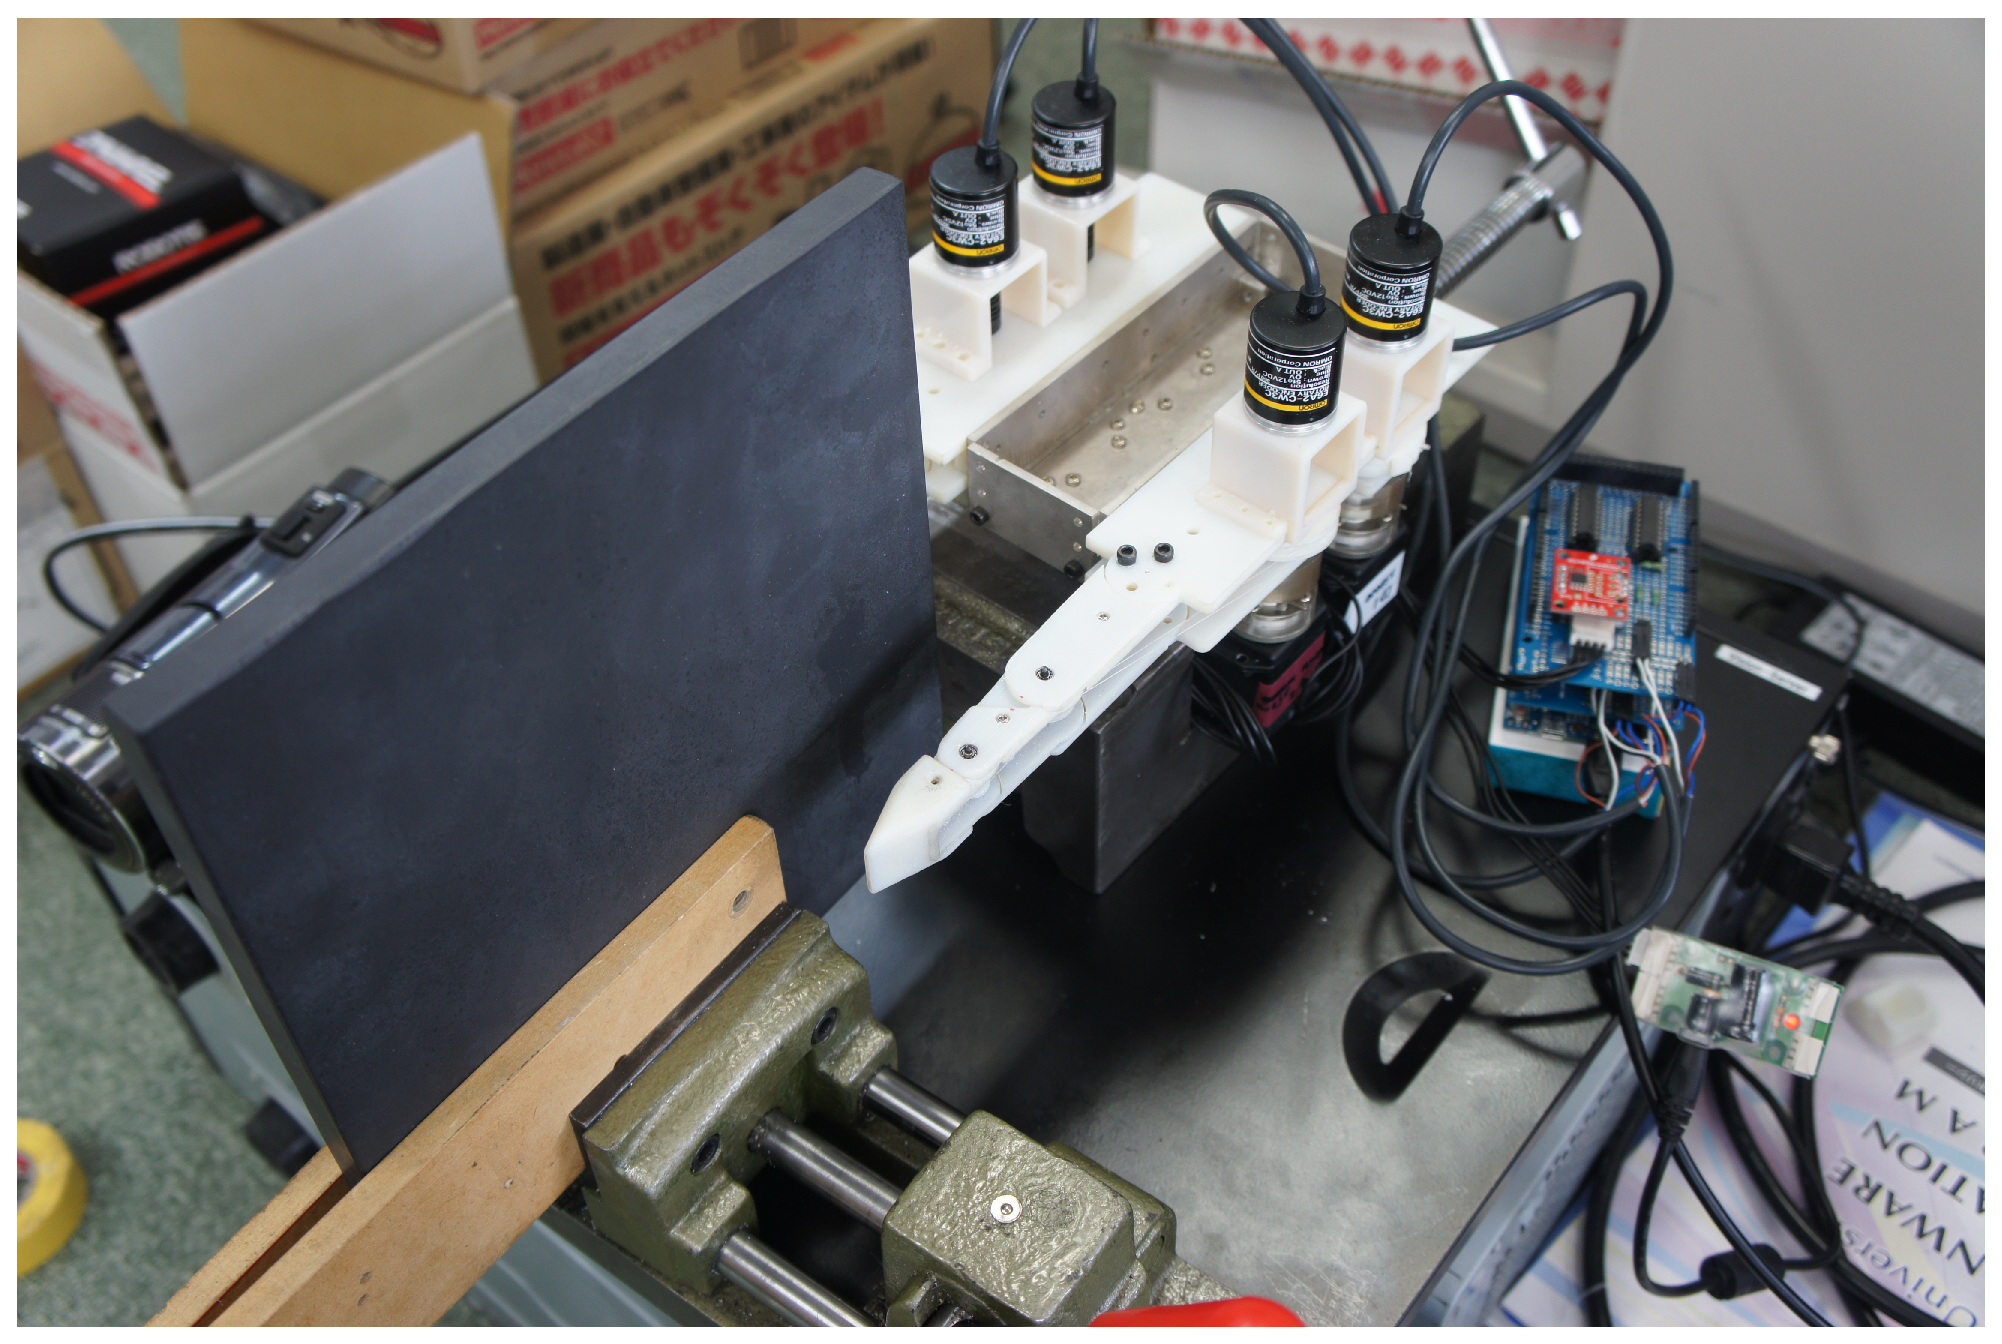
\includegraphics[width=.60\textwidth]{./figure/JPG/experiment2.eps}
% 				\caption{実験風景}
% 				\label{pic:experiment}
% 			\end{figure}

% 			% 実験は,開発したフィンガと,接触させる物体を万力で固定し,接触する物体と指先の角度を固定し,て行った.
% 			実験(1)として,まず,$\theta_2=15^{\circ}$で,$s=0.6, s=0.8$に対して,十分に大きいバイアス張力でフィンガを動作させ始め,バイアス張力を徐々に緩めていき,緩みの条件の値を下回ったときに,分岐腱が緩むことを確認した.

% 			次に,実験(2)から(5)として,実験において,分岐腱に実際に緩みが起こったバイアス張力の値に対して,その周辺の値でフィンガを動作させ始め,実際にどの程度のバイアス張力で緩みが生じるのかを観察した.
% 			緩み条件は,前述のように,関節の角度と,指先の力に関係して変化するため,実験では,

% 			\begin{itemize}
% 				\item 関節の角度と指先の力を固定し,さまざまなバイアス張力を加えたときのフィンガの挙動を確認した.
% 				\item その後,角度はそのままに,指先の力を変えて同様の実験を行い,指先の力に対する緩み条件の違いを確認した.
% 				\item 最後に,ある大きさの指先の力に対して,関節の角度を変え,フィンガの動きを確認した.
% 			\end{itemize}

% 			実験(2)から(5)でパラメータとして実験した,角度と指先の力の値の組は,表\ref{tab:slack_experiment_parameter}にまとめた通りである.
% 			これらのパラメータに対して,バイアス張力を変化させながら,腱が緩むかどうか確認した.

% 			\begin{table}
% 				\centering
% 				\caption{実験におけるパラメータ}
% 				\label{tab:slack_experiment_parameter}
% 				\begin{tabular}{|c||c|c|c|} \hline
% 					 & 関節2の角度$\theta_2$[deg] & 指先の力$s$[N] & 緩み条件の計算結果 \\ \hline
% 					(2) &  & 0.3 & 1.12 \\ \cline{3-4}
% 					(3) & 15 & 0.6 & 2.25 \\ \cline{3-4}
% 					(4) &  & 0.8 & 3.00 \\ \hline
% 					(5) & 25 & 0.6 & 1.95 \\ \hline
% 				\end{tabular}
% 			\end{table}

% 			実験手順は以下の通りである.

% 			\begin{enumerate}
% 				\item 腱張力が0の状態から,バイアス張力をかけ,フィンガを伸びた状態で安定させる.
% 				\item 指先に発生させる力に対応する関節トルクが発生するように,腱に張力をかけ,フィンガを動かす.
% 				\item 所定の角度で指先が接触するように固定した,摩擦の少ない板に指先を当てて,力をかけさせる.
% 				\item バイアス張力を徐々に小さくしていき,腱の緩みを観察する.
% 				\item 腱が緩み,関節の連動が崩れるか,計算された駆動軸のトルクが負になるまで,フィンガを動作させ,元の伸ばした状態に戻す.
% 			\end{enumerate}

% 			また,腱2と腱1の間のバイアス張力の比は,計算通りであれば,$1:1.8$になれば関節にトルクは発生せず,フィンガは運動しないはずである.
% 			しかし,実際には,ねじりばねの初期変位を0に設定することの難しさなどの要因から,この比のバイアス張力をかけるとフィンガが運動してしまう.
% 			フィンガの運動において,トルクの発生しない腱張力は重要であるため,理論式とは一致しないが,これは,調整して釣り合いのとれた値を探す必要のある部分である.
% 			そこで,実験を始める前に,$\theta_1,\theta_2=0$になるように位置制御を行い,フィンガが伸びた状態で安定させ,このときの腱2の腱張力を1とした場合の腱1の腱張力を求め,これを前述のバイアス張力の比として利用することとした.
% 			この比は,測り直す度に微妙なずれが生じるため,(1)から(3)の実験中,この比の値は一定とし,実験結果に与える影響に大差がつかないようにした.
% 			ただし,実験(4)は,(3)までと別の日に行ったため,腱張力の比は,同じではない.
% 			しかし,実験の前に,フィンガを安定させて腱張力の比をとる作業を行っている.

% 		% subsection process_of_experiment (end)

% 	% section slack_experiment (end)

% 	\section{結果・考察} % (fold)
% 	\label{sec:slack_conclusion}
% 		% 実験の結果を以下の図\ref{fig:slack_conclusion1},\ref{fig:slack_conclusion2},\ref{fig:slack_conclusion3},\ref{fig:slack_conclusion4}の通りである.
% 		% また,実験時のフィンガの動きの例を図\ref{pic:example_slack}に示す.

% 		% グラフは,横軸が時間[ms]で,縦軸は,バイアス張力の大きさ[N]とエンコーダが測定した駆動軸の回転角度[deg]である.
% 		% バイアス張力は,式(\ref{eq:independent-f})における$f_b$の値であり,腱2のバイアス張力の大きさに相当する.
% 		% エンコーダの角度は,駆動軸プーリの角度変位を測定しているロータリエンコーダの値そのままである.
% 		% フィンガが物体に接触し,腱に緩みがないとき,フィンガは動かないので,腱の変位は起こらずエンコーダの角度値も一定になるはずである.
% 		% 緩みが生じたとき,フィンガは,緩んでいない腱2本で駆動するため,フィンガには動きが生じ,腱が移動する.
% 		% したがって,駆動軸のエンコーダの値が,釣り合いの状態から変化した時点で腱が緩んでいると考えられる.
% 		% このときの,バイアス張力$f_b$の値を分岐腱が緩まないための限界値だと考える.
% 		% % ここで,この角度は,エンコーダ1とエンコーダ2の角度の値からそれぞれ計算した,連動状態での関節1の角度の差をとったものである.
% 		% % フィンガが物体に接触し,腱に緩みがないとき,腱は移動しないはずであるので,この角度の差には変化がない.
% 		% % エンコーダの値が増えた→腱が巻き取られた,緩みはじめた→,少しでも動き始めたところで緩んでいる可能性.

	

% 		まず,関節の角度を$\theta_2=15^{\circ}$,フィンガの出す力を$s=0.6$と$s=0.8$として,十分に大きなバイアス張力でフィンガを動かし始めたときの実験結果を,図\ref{fig:slack_conclusion}に示す.
% 		また,実験時のフィンガの動きの例を図\ref{pic:example_slack}に示す.

% 		\begin{figure}[tbhp]
% 		\centering
% 			\subfigure[$s=0.6$\label{fig:r60b500}]{\includegraphics*[width=.49\textwidth]{./pdf/2320t15r60b500shadow.pdf}}
% 			\subfigure[$s=0.8$\label{fig:r80b450}]{\includegraphics*[width=.49\textwidth]{./pdf/2425t15r80b450shadow.pdf}}
% 			\caption{実験結果(1)$\theta_2=15^{\circ}$}
% 			\label{fig:slack_conclusion}
% 		\end{figure}

% 		\begin{figure}[tbhp]
% 			\centering
% 			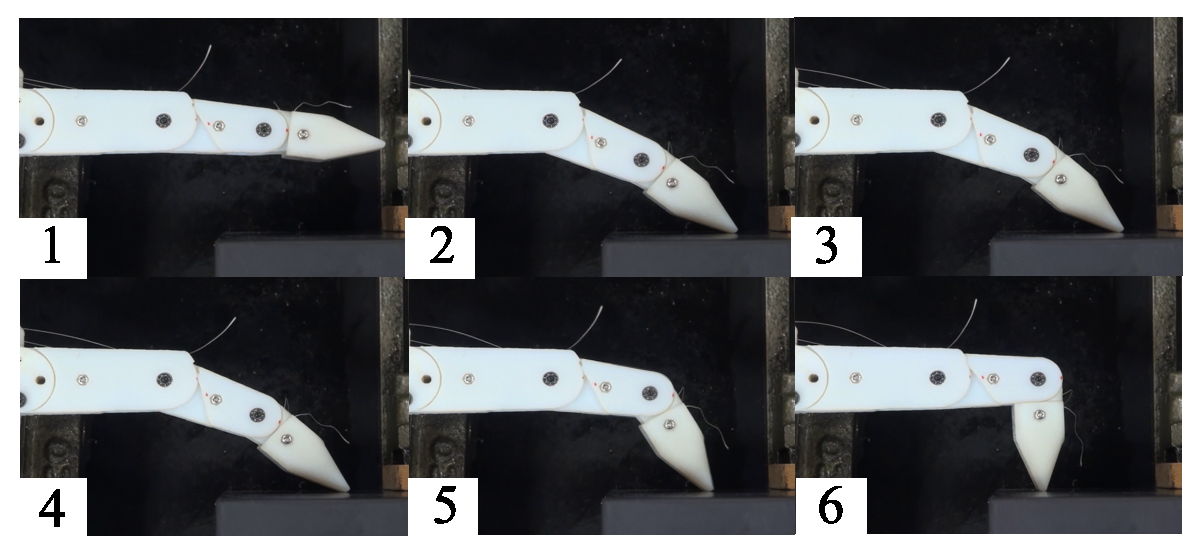
\includegraphics[width=\textwidth]{./figure/frame1733r60b180.pdf}
% 			\caption{実験時にフィンガの腱が緩む様子}
% 			\label{pic:example_slack}
% 		\end{figure}

% 		グラフは,横軸が時間[ms]で,縦軸は,バイアス張力の大きさ[N]とエンコーダが測定した駆動軸の回転角度[deg]である.
% 		バイアス張力は,式(\ref{eq:independent-f})における$f_b$の値であり,腱2のバイアス張力の大きさに相当する.
% 		エンコーダの角度は,分岐腱である腱1を駆動しているプーリに直結されている,ロータリエンコーダの測定値から計算した,駆動軸の角度変位である.
% 		エンコーダの値は腱1が伸びたとき,つまり,連動状態のフィンガが屈曲方向に動いたときに,増加する.
% 		ここで,グラフでは,バイアス張力が分岐腱の緩む条件となる,下限値thresholdを点線で示し,これを下回っている部分に,グレーの色づけを行っている.

	As graph shows, tendon1s get slack and finger movement causes increasement of the value of the encoder after bias tensile force $f_b$ fall short of the limit to keep tendon 1s's tensile force positive.
	It is verified that the slack of one of the branching tendon is caused by the value of bias tensile force.
% 		グラフから分かるように,徐々に下げていったバイアス張力$f_b$の値が,腱1sの張力を正に保つことができる下限値を下回ると,腱が緩み,フィンガが動いてエンコーダの値が増加している.
% 		このように,バイアス張力により,分岐腱の緩みを生じさせることができることがわかった.

	
% 		エンコーダによる駆動軸の角度を観測すると,フィンガに大きな動作がない間も,値が徐々に増加していることが観察できる.
% 		この値の増加は,駆動軸が腱が緩む方向に微小に回転していることを示しているが,本来,フィンガの関節が動いていない間は,駆動軸に回転は生じないはずである.
% 		この原因としては,バイアス張力の現象によって腱張力が減少することで,値の変化が起こっていることから,駆動軸から腱にかけての間にわずかな弾性が存在していることが考えられる.
% 		弾性の要因としては,腱に使用した糸のわずかな弾性のほかに,駆動軸における腱の固定や関節のプーリへの腱の食い込みなどが考えられる,
% 		今後,これらの要因をできうる限り排除することが望まれる.

% 		% フィンガが物体に接触し,腱に緩みがないとき,フィンガは動かないので,腱の変位は起こらずエンコーダの角度値も一定になるはずである.
% 		% 緩みが生じたとき,フィンガは,緩んでいない腱2本で駆動するため,フィンガには動きが生じ,腱が移動する.
% 		% したがって,駆動軸のエンコーダの値が,釣り合いの状態から変化した時点で腱が緩んでいると考えられる.
% 		% このときの,バイアス張力$f_b$の値を分岐腱が緩まないための限界値だと考える.

% 		実際に腱が緩んだ周辺の値に対して,どの程度のバイアス張力で腱がゆるみ始めるのか,確認するため,実験(2)から(5)を行った.
% 		実験の結果は,以下の図\ref{fig:slack_conclusion1},\ref{fig:slack_conclusion2},\ref{fig:slack_conclusion3},\ref{fig:slack_conclusion4}の通りである.

% 		\begin{figure}[tbh]
% 		\centering
% 			\subfigure[$f_b=0.8$\label{fig:r30b80}]{\includegraphics*[width=.48\textwidth]{./pdf/r30/1805r30b80.pdf}}
% 			\subfigure[$f_b=0.9$\label{fig:r30b90}]{\includegraphics*[width=.48\textwidth]{./pdf/r30/1811r30b90.pdf}}
% 			\subfigure[$f_b=1.0$\label{fig:r30b100}]{\includegraphics*[width=.48\textwidth]{./pdf/r30/1813r30b100.pdf}}
% 			\subfigure[$f_b=1.1$\label{fig:r30b110}]{\includegraphics*[width=.48\textwidth]{./pdf/r30/1817r30b110.pdf}}
% 			\caption{実験結果(2)$\theta_2=15^{\circ},s=0.3$}
% 			\label{fig:slack_conclusion1}
% 		\end{figure}

% 		\begin{figure}[tbh]
% 		\centering
% 			\subfigure[$f_b=1.6$\label{fig:r60b160}]{\includegraphics*[width=.48\textwidth]{./pdf/r60/1728r60b160.pdf}}
% 			\subfigure[$f_b=1.8$\label{fig:r60b180}]{\includegraphics*[width=.48\textwidth]{./pdf/r60/1726r60b180.pdf}}
% 			\subfigure[$f_b=2.0$\label{fig:r60b200}]{\includegraphics*[width=.48\textwidth]{./pdf/r60/1724r60b200.pdf}}
% 			\subfigure[$f_b=2.2$\label{fig:r60b220}]{\includegraphics*[width=.48\textwidth]{./pdf/r60/1717r60b220.pdf}}
% 			\caption{実験結果(3)$\theta_2=15^{\circ},s=0.6$}
% 			\label{fig:slack_conclusion2}
% 		\end{figure}

% 		\begin{figure}[tbh]
% 		\centering
% 			\subfigure[$f_b=2.4$\label{fig:r80b240}]{\includegraphics*[width=.48\textwidth]{./pdf/r80/1848r80b240.pdf}}
% 			\subfigure[$f_b=2.6$\label{fig:r80b260}]{\includegraphics*[width=.48\textwidth]{./pdf/r80/1854r80b260.pdf}}
% 			\subfigure[$f_b=2.8$\label{fig:r80b280}]{\includegraphics*[width=.48\textwidth]{./pdf/r80/1859r80b280.pdf}}
% 			\subfigure[$f_b=3.0$\label{fig:r80b300}]{\includegraphics*[width=.48\textwidth]{./pdf/r80/1908r80b300.pdf}}
% 			\caption{実験結果(4)$\theta_2=15^{\circ},s=0.8$}
% 			\label{fig:slack_conclusion3}
% 		\end{figure}

% 		\begin{figure}[tbh]
% 		\centering
% 			\subfigure[$f_b=1.4$\label{fig:t25b140}]{\includegraphics*[width=.48\textwidth]{./pdf/t25/1313t25r60b140.pdf}}
% 			\subfigure[$f_b=1.5$\label{fig:t25b150}]{\includegraphics*[width=.48\textwidth]{./pdf/t25/1317t25r60b150.pdf}}
% 			\subfigure[$f_b=1.7$\label{fig:t25b170}]{\includegraphics*[width=.48\textwidth]{./pdf/t25/1321t25r60b170.pdf}}
% 			\subfigure[$f_b=1.9$\label{fig:t25b190}]{\includegraphics*[width=.48\textwidth]{./pdf/t25/1327t25r60b190.pdf}}
% 			\caption{実験結果(5)$\theta_2=25^{\circ},s=0.6$}
% 			\label{fig:slack_conclusion4}
% 		\end{figure}

% 		グラフには,伸展側の分岐腱を駆動するプーリの角度変位をencoder1として,屈曲側の腱を駆動するプーリの角度変位をencoder2としてプロットしている.
% 		グラフを観察すると,腱が緩むバイアス張力の値は,おおよそ表\ref{tab:result_slack}のようになっている.
% 		% ここで,グラフでは,エンコーダの値が変化し,腱が緩んでいるのではないかと思われる部分に,グレーの色づけを行っている.
% 		腱が緩むと,フィンガは,図\ref{pic:example_slack}のような大きな動作をし,この動きは,グラフ上でもエンコーダの値の大きな変化として観察できる.
% 		しかし,図\ref{pic:example_slack}では分かりにくいが,実験では,フィンガが大きく動作する前に腱がたるみ,緩みが生じていることが,観察できた.
% 		このように,フィンガの動作が生じる前に腱の緩みは生じており,グラフの色づけは,この現象を考慮して,エンコーダの値の小さな変化を参考に,腱が緩んだと思われるときのバイアス張力の値を目測し,記載している.
% 		また,たるみの観察でも,緩む腱の張力が0になった瞬間は分からないため,実際には,もっと早く,バイアス張力が大きい段階で,腱には張力がかからなくなっている可能性もある.
% 		これを観察するためには,腱張力を測定するセンサが必要になる.

% 		\begin{table}[tbhp]
% 			\centering
% 			\caption{結果}
% 			\label{tab:result_slack}
% 			\begin{tabular}{|c||c|c|c|} \hline
% 				 & グラフから読み取った,緩んだときのバイアス張力[N] & 計算結果[N] & 実験と計算の差\\ \hline \hline
% 				(1) & 0.7 〜 0.8 & 1.12 & 約0.4	\\ \hline
% 				(2) & 1.6 〜 1.8 & 2.25 & 約0.5	\\ \hline
% 				(3) & 2.3 〜 2.4 & 3.00 & 約0.6	\\ \hline
% 				(4) & 1.1 〜 1.4 & 1.92 & 約0.7	\\ \hline
% 			\end{tabular}
% 		\end{table}

% 		グラフから読み取れる実験結果を計算値と比べると,総じて低い値となっていることが分かる.
% 		また,その差は,0.5程度とどのパラメータにおける実験でも似た値となっている.
% 		この差の値は,バイアス張力の値と比べて十分に小さい値であるとは言えないため,緩み条件の計算方法に多少の問題がある可能性もある.
% 		しかし,傾向としては,実験間の結果の値の推移は,計算結果と似通っている.
% 		そのため,この差は,実験環境や,計算において無視した要素が主たる要因であると考えることができる.

% 		特に大きな要素として,フィンガと物体の接触面において,摩擦を無視したことがあげられる.
% 		この摩擦の存在を考慮すると,フィンガの腱が緩み,物体表面を滑るような動きをするためにより大きな力が必要になる.
% 		腱が緩んだことによるフィンガの動き出しがこの摩擦により遅れるとすると,腱のたるみ,フィンガの動きは,実際の件の緩みよりも遅れることが考えられ,計算との差が生じる原因となりうる.
% 		また,フィンガの関節,駆動軸における摩擦についても考慮していない.
% 		軸の摩擦は,接触面の摩擦と同様,フィンガの動作を阻害し,腱の緩みを遅らせると思われる.
% 		摩擦の影響が観察できるのは,図\ref{fig:slack_conclusion1}である.
% 		$f_b=0.8$で動作させた,図\ref{fig:r30b80}では,0.8にかなり近い値で緩みが生じてフィンガが動いているのに対して,これよりも大きい$f_b$で動かし始めている他の3パラメータでは,0.7に近い値で緩みが生じている.
% 		これは,緩み条件に近い値では,フィンガが板に接触してすぐに動きだすのに対して,それよりも大きい値だと,一旦運動が止まってから再度動き出すため,同摩擦に比べて大きい静止摩擦が生じているからだと考えられる.
% 		これらの,計算では簡単のため考慮しなかったさまざまな力学的要因について,実際にロボットを制御する際には,その影響を勘案しながら制御システムを構築する必要がある.

% 		さらに,実験手順の説明で述べたように,腱2と腱1の間のバイアス張力の比の問題と調整についての問題も存在する.
% 		実験では,データを取る前に,フィンガが動かないような腱張力の比を探して,この値を利用している.
% 		しかし,ねじりばねの初期位置の設定により,この値は大きく変動し,また,関節の摩擦の存在のため,フィンガが動かないような腱張力の比には幅がある.
% 		これらの影響を除くことは,現在のシステムでは難しく,ロボットの改善が望まれる点である.

% 		また,フィンガの関節間の長さ,関節の角度などの測定誤差も考えられる.
% 		関節間の長さに,実際よりも短い値を用いていると,腱が緩むバイアス張力の値は,実際よりも大きく計算されてしまう.
% 		また,フィンガが指先に出す力に必要な関節トルクが小さく計算されてしまうため,指定した力よりも小さな力しかかからない.
% 		フィンガの力が小さくなると,腱が緩むバイアス張力の値も小さくなる.
% 		したがって,関節間の長さが,実際よりも短く測定されればされるほど,緩み条件の値と実際に緩んだときのバイアス張力との差は広がることになる.
% 		関節の角度も,緩み条件とフィンガの出す力に必要な関節トルク両方に影響を与えるので,これらの要素の測定誤差が実験結果に現れている可能性がある.

% 		今後,以上のような要素について考慮し,再実験も視野に入れて研究を進めることが望まれる.

% 		% また,実験を行っている最中に,腱のプーリなどとの固定部分が緩んで腱の長さが微小に変わっていることも考えられ,実験の

% 		% これらの実験結果から,バイアス張力が十分に大きい場合には,関節が連動したまま,指先に力を発生させることができ,バイアス張力が小さい場合には,関節の連動が外れてフィンガが動くことを示すことができた.
% 		% 実験結果と計算には差異が生じているが,バイアス張力の設定により意図的に関節の連動を操作できるフィンガ,というコンセプトは実現できたと考える.
% 		% 今後は,実際に,グリッパとして物体を把持したときに,腱が緩んだ状態で物体操作を実現できるか,という問題を検証する必要がある.

% 	% section slack_conclusion (end)

% %\clearpage
% % chapter verification (end)



% section verification (end)








% \begin{verbatim}
% \begin{thebibliography}{}  % (do not forget {})
% .
% .
% \bibitem[1982]{clar:eke}
% Clarke, F., Ekeland, I.:
% Nonlinear oscillations and boundary-value problems for
% Hamiltonian systems.
% Arch. Rat. Mech. Anal. 78, 315--333 (1982)
% .
% .
% \end{thebibliography}
% \end{verbatim}
% {\itshape Sample Output}
% \bibauthoryear
%

\end{document}
